%to have line numbers
%\RequirePackage{lineno}
\documentclass[10pt, letterpaper]{article}      
\usepackage[margin=.1cm,font=small,labelfont=bf]{caption}[2007/03/09]
%\usepackage{endnotes}
%\let\footnote=\endnote
\usepackage{setspace}
\usepackage{longtable}                        
\usepackage{anysize}                          
\usepackage{natbib}                           
%\bibpunct{(}{)}{,}{a}{,}{,}                   
\bibpunct{(}{)}{,}{a}{}{,}                   
\usepackage{amsmath}
\usepackage[% draft,
pdftex]{graphicx} %draft is a way to exclude figures                
\usepackage{epstopdf}
\usepackage{hyperref}                             % For creating hyperlinks in cross references


% \usepackage[margins]{trackchanges}

% \note[editor]{The note}
% \annote[editor]{Text to annotate}{The note}
%    \add[editor]{Text to add}
% \remove[editor]{Text to remove}
% \change[editor]{Text to remove}{Text to add}

%TODO make it more standard before submission: \marginsize{2cm}{2cm}{1cm}{1cm}
\marginsize{1cm}{1cm}{.5cm}{.5cm}%{left}{right}{top}{bottom}   
					          % Helps LaTeX put figures where YOU want
 \renewcommand{\topfraction}{1}	                  % 90% of page top can be a float
 \renewcommand{\bottomfraction}{1}	          % 90% of page bottom can be a float
 \renewcommand{\textfraction}{0.0}	          % only 10% of page must to be text

 \usepackage{float}                               %latex will not complain to include float after float

\usepackage[table]{xcolor}                        %for table shading
\definecolor{gray90}{gray}{0.90}
\definecolor{orange}{RGB}{255,128,0}

\renewcommand\arraystretch{.9}                    %for spacing of arrays like tabular

%-------------------- my commands -----------------------------------------
\newenvironment{ig}[1]{
\begin{center}
 %\includegraphics[height=5.0in]{#1} 
 \includegraphics[height=3.3in]{#1} 
\end{center}}

 \newcommand{\cc}[1]{
\hspace{-.13in}$\bullet$\marginpar{\begin{spacing}{.6}\begin{footnotesize}{#1}\end{footnotesize}\end{spacing}}
\hspace{-.13in} }

%-------------------- END my commands -----------------------------------------



%-------------------- extra options -----------------------------------------

%%%%%%%%%%%%%
% footnotes %
%%%%%%%%%%%%%

%\long\def\symbolfootnote[#1]#2{\begingroup% %these can be used to make footnote  nonnumeric asterick, dagger etc
%\def\thefootnote{\fnsymbol{footnote}}\footnote[#1]{#2}\endgroup}	%see: http://help-csli.stanford.edu/tex/latex-footnotes.shtml

%%%%%%%%%%%
% spacing %
%%%%%%%%%%%

% \abovecaptionskip: space above caption
% \belowcaptionskip: space below caption
%\oddsidemargin 0cm
%\evensidemargin 0cm

%%%%%%%%%
% style %
%%%%%%%%%

%\pagestyle{myheadings}         % Option to put page headers
                               % Needed \documentclass[a4paper,twoside]{article}
%\markboth{{\small\it Politics and Life Satisfaction }}
%{{\small\it Adam Okulicz-Kozaryn} }

%\headsep 1.5cm
% \pagestyle{empty}			% no page numbers
% \parindent  15.mm			% indent paragraph by this much
% \parskip     2.mm			% space between paragraphs
% \mathindent 20.mm			% indent math equations by this much

%%%%%%%%%%%%%%%%%%
% extra packages %
%%%%%%%%%%%%%%%%%%

\usepackage{datetime}


\usepackage[latin1]{inputenc}
\usepackage{tikz}
\usetikzlibrary{shapes,arrows,backgrounds}


%\usepackage{color}					% For creating coloured text and background
%\usepackage{float}
\usepackage{subfig}                                     % for combined figures

\renewcommand{\ss}[1]{{\colorbox{blue}{\bf \color{white}{#1}}}}
\newcommand{\ee}[1]{\endnote{\vspace{-.10in}\begin{spacing}{1.0}{\normalsize #1}\end{spacing}\vspace{.20in}}}
\newcommand{\emd}[1]{\ExecuteMetaData[/tmp/tex]{#1}} % grab numbers  from stata

%TODO before submitting comment this out to get 'regular fornt'
\usepackage{sectsty}
\allsectionsfont{\normalfont\sffamily}
\usepackage{sectsty}
\allsectionsfont{\normalfont\sffamily}
\renewcommand\familydefault{\sfdefault}

\usepackage[margins]{trackchanges}
\usepackage{rotating}
\usepackage{catchfilebetweentags}
%-------------------- END extra options -----------------------------------------
\date{Draft: {}\today}
\title{
  XXX
}
\author{
Adam Okulicz-Kozaryn\thanks{EMAIL: adam.okulicz.kozaryn@gmail.com
  \hfill I thank XXX.  All mistakes are mine.} \\
{\small Rutgers - Camden}
}

\begin{document}

%%\setpagewiselinenumbers
%\modulolinenumbers[1]
%\linenumbers

\bibliographystyle{/home/aok/papers/root/tex/ecta}
\maketitle
\vspace{-.4in}
\begin{center}

\end{center}


\begin{abstract}
\noindent
\end{abstract}
\vspace{.15in} 
\noindent{\sc keywords:  XXX}
%\vspace{-.25in} 

\begin{spacing}{1.4} %TODO MAYBE before submission can make it like 2.0
\rowcolors{1}{white}{gray90}

\section{most current stuff}

\ref{couWvsLsEleHHgdp} shows Average electricity consumption per electrified household, kWh, from World
Energy Council (1990-2011) (\url{http://www.wec-indicators.enerdata.eu/household-electricity-use.html}), which are also averaged. 
% energy use from World Bank (\url{http://data.worldbank.org/indicator})
   US consumes
in its residential sector about more than 3 times the median.%sum eleHH
                                %if yr==2011 & c=="USA", det for FULL sample 
From first panel, it appears
 as if there is a positive relationship, but it is simply due to wealth. Simply,
 developed countries consume more energy than developing countries, and we know
 that in a cross-section, wealthier countries are happier. The second panel
 measures on x-axis energy intensity of gross domestic product (GDP)
 (energy/GDP). Here, the relationship is opposite--countries that  consume less
 energy per unit of wealth are happier. In other words, the less energy use
 given income level, the more happiness. We speculate that to acheive greater happiness we
 do not necessarily need to increase GDP keeping energy constant; we could stop
 growing GDP and decrease energy use. For instance, the Netherlands (NLD) is
 happy, developed and energy efficient. China (CHN) is developing and medium
 happy, but consumes more energy per GDP than developed and happier USA does.  
Latin America countries, pose a puzzle for happiness researchers-they are
relatively poor and yet quite happy, but they also  use very liitle  energy per
their GDP and have simialr energy inetsity of GDP as the US. Next, we zoom in on
US states and counties.
% also see http://www.ritholtz.com/blog/2010/06/oil-consumption-around-the-world/ 

\begin{figure}[H]
 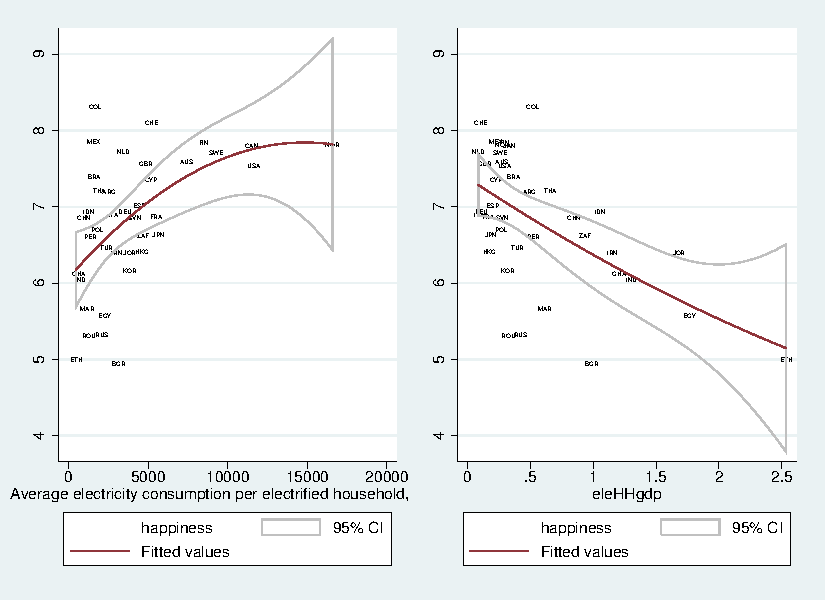
\includegraphics[width=6in]{graphsAndTables/couWvsLsEleHHgdp.pdf}\centering
 \caption{Happiness against average electricity consumption per electrified
   household, kWh.}\label{couWvsLsEleHHgdp}
\end{figure}
{\scriptsize Note: Country codes are in table \ref{ls} in supplementary
  material. If country was observed in more than one year, the data were averaged.}



Well, true energy look positive, but so what ! does it mean more energymore
happiness. no. it is quadratic!!! so it levels off at around 4k of energy
use--beyond that anergy use does not seem to help much wiuth happiness; like
with income--it also levels off at country or regional levble (my paper!)

it is interesting that the ere is positive quadratic relationship in rich
countries and negative in poor countries...the cutoff point is at 10k of pcgdp.

note: happiness and gdp were averaged over time: in wvs there are couple years;
in mannheim there are 30years so not sure if averaging is a great idea in
mannheim; but if each country-year plotted, it's quadratic also 


\begin{figure}[H]
 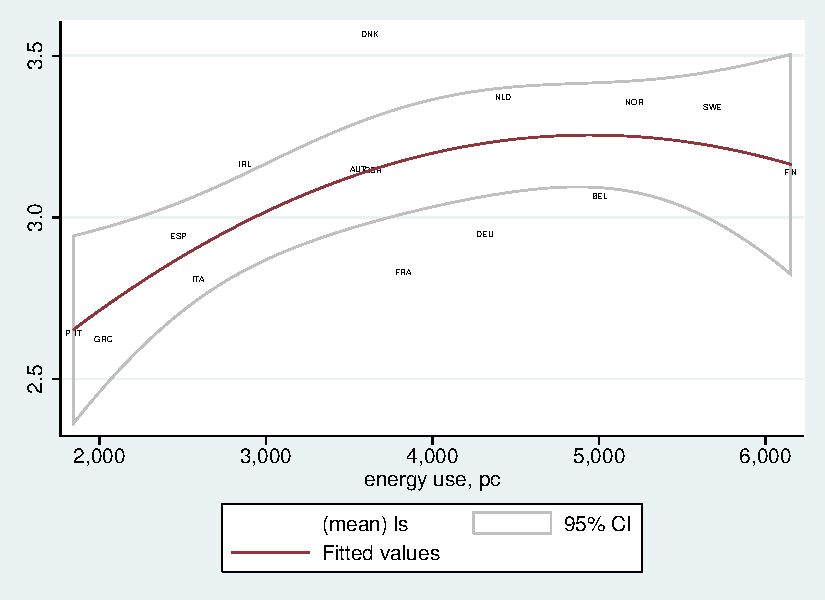
\includegraphics[height=3in]{graphsAndTables/couLsEne.pdf}\centering
\caption{couLsEne.pdf Eurobarometer dataset for west european (rich countries)}\label{couLsEne.pdf}
\end{figure}
{\scriptsize Note: Country codes are in table \ref{ls} in supplementary
  material. If country was observed in more than one year, the data were averaged.}

\begin{figure}[H]
 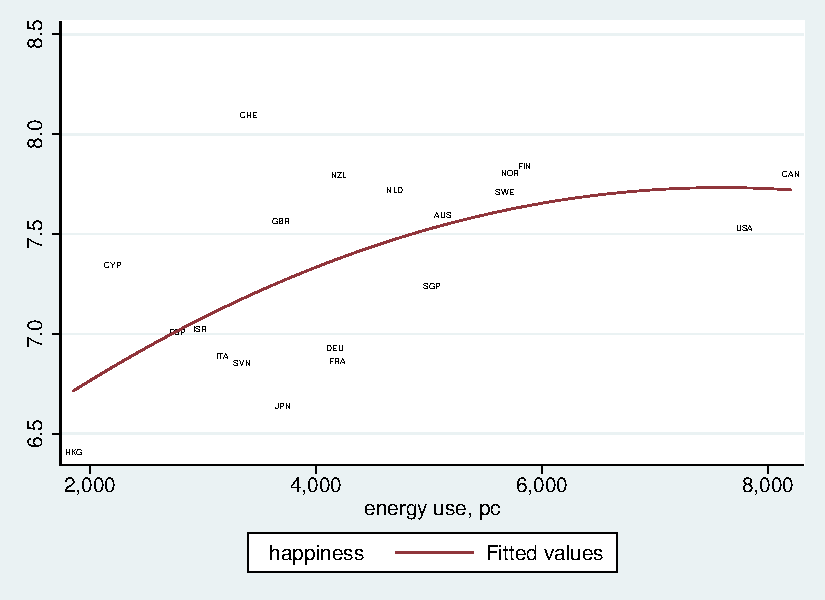
\includegraphics[height=3in]{graphsAndTables/couWvsLsEne.pdf}\centering
\caption{World Values Survey Data data; countries$>$10k pcgdp couWvsLsEne.pdf}\label{couWvsLsEne.pdf}
\end{figure}
{\scriptsize Note: Country codes are in table \ref{ls} in supplementary
  material. If country was observed in more than one year, the data were averaged.}


\begin{figure}[H]
 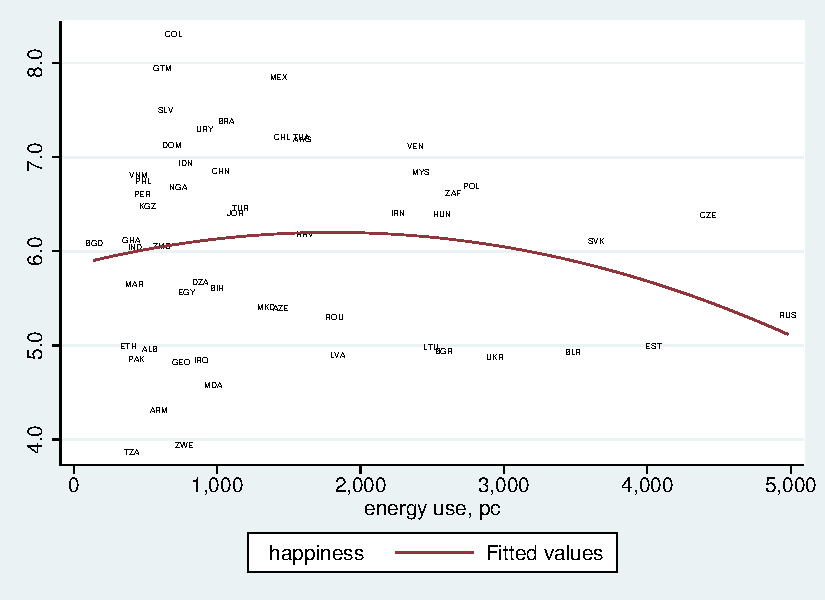
\includegraphics[height=3in]{graphsAndTables/couWvsLsEneLT10kGDP.pdf}\centering
\caption{couWvsLsEneLT10kGDP.pdf World values survey data country level for
  countries lt 10k pcgdp--btw this doesn't make sense--should be the other way
  round--more ebergy consumption is helpful in poor countries, not rich onese
  e.g. as per \cite{mazur11}}\label{couWvsLsEneLT10kGDP.pdf}
\end{figure}
{\scriptsize Note: Country codes are in table \ref{ls} in supplementary
  material. If country was observed in more than one year, the data were averaged.}


\begin{figure}[H]
 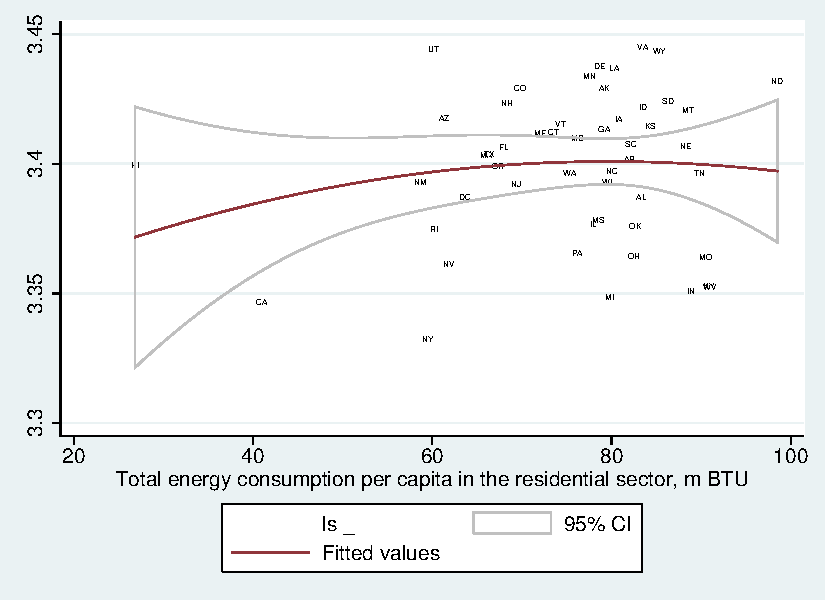
\includegraphics[height=3in]{graphsAndTables/lfTERPBls.pdf}\centering
\caption{lfTERPBls.pdf residential energy consumptionm; no relationship here !
  except that hawaii is warm and doesn't consume much and california is green!
  so now zooming in on california :)}\label{grComTETPBgdp}
\end{figure}
{\scriptsize TODO Note: Country codes are in table \ref{ls} in supplementary
  material. If country was observed in more than one year, the data were averaged.}


\begin{figure}[H]
 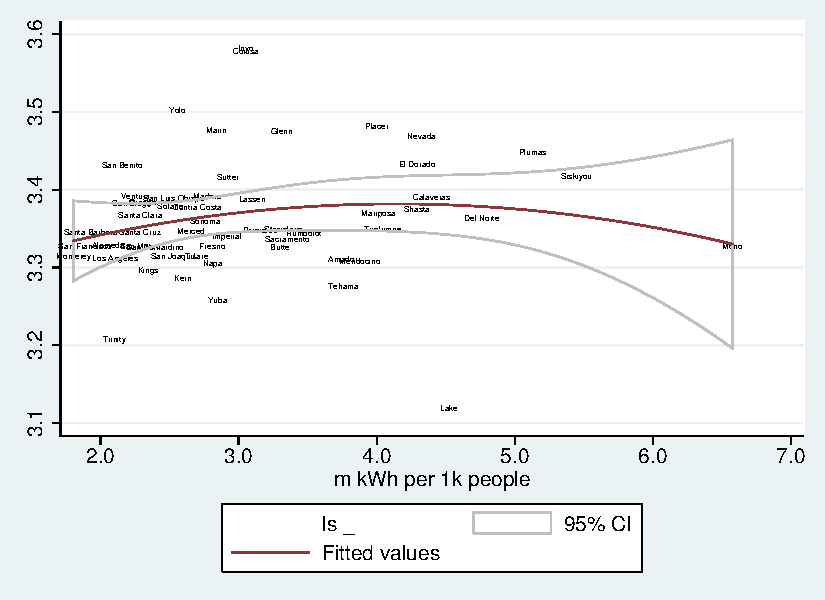
\includegraphics[height=3in]{graphsAndTables/lfELERESls.pdf}\centering
\caption{residential energy use; nothing reallyu here...wonde why Mono uses so much!}\label{}
\end{figure}
{\scriptsize TODO Note: Country codes are in table \ref{ls} in supplementary
  material. If country was observed in more than one year, the data were averaged.}

\begin{figure}[H]
 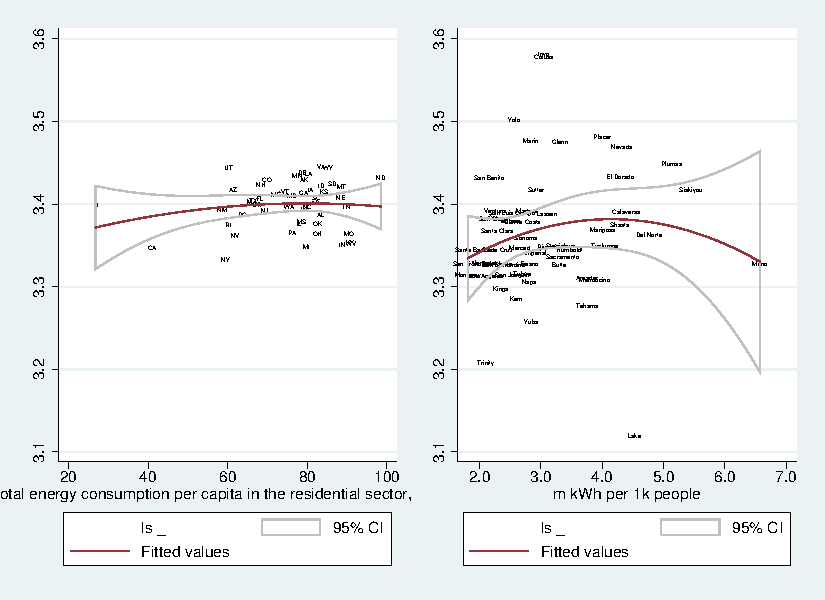
\includegraphics[width=6in]{graphsAndTables/stateCa.pdf}\centering
\caption{WVS all countries, avergaed over time;; in this second step we explore
at state and county lev and nothing there whether with or without gdp--and
importantly as at ctry lev also energy intencsity attenuates slope albeit much
less dramatcally}\label{stateCa}
 \end{figure} {\scriptsize Note: Country codes are in table \ref{ls} in supplementary material. If country was observed in more than one year, the data were averaged. }


\subsection{Energy intensity of gross domestic product (GDP) (energy/GDP)}

\url{http://en.wikipedia.org/wiki/Energy_intensity}:
High energy intensities indicate a high price or cost of converting energy into GDP.
 
\begin{figure}[H]
 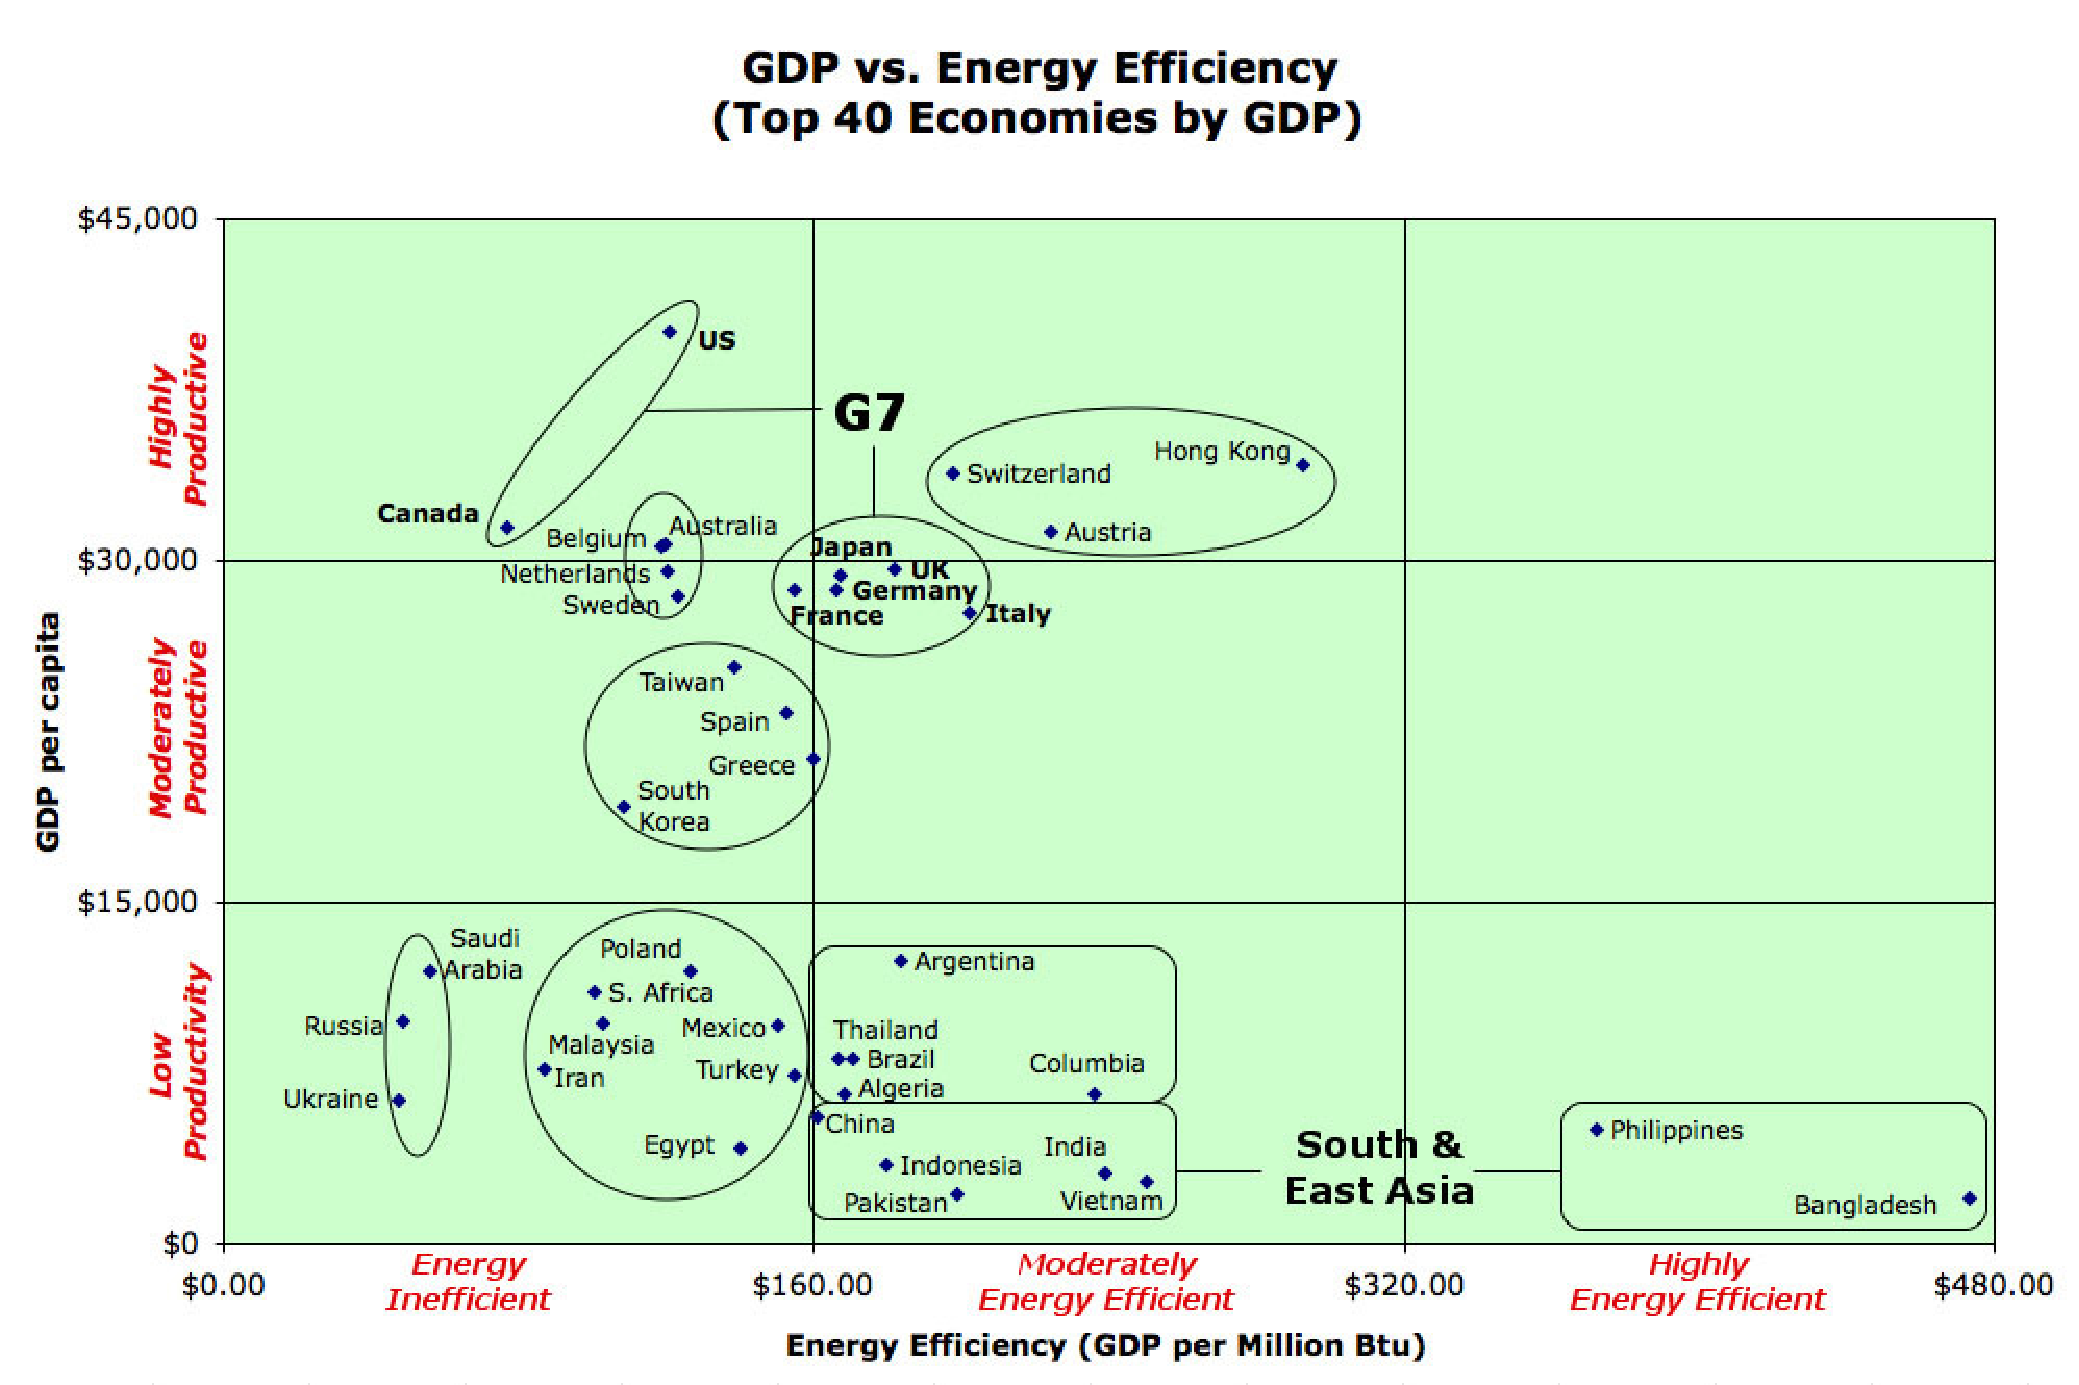
\includegraphics[height=5in]{graphsAndTables/Gdp-energy-efficiency.pdf}\centering
\caption{a cool graph from wikipedia :)}\label{}
\end{figure}
and can also use energy intensity PPP adjusted--see above wikipedia article and \url{http://en.wikipedia.org/wiki/List_of_countries_by_energy_intensity}

There is not much relatyionship between happpiness and energy use, but there is
even less if controlling for GDP--energy use correlates with GDP and it if nit
controlling for GDP then it proxies it and then results are spurioius and what
we see is the effect of GDP, not energy use.  
To alleviate that problem we could have controlled for GDP. But we can do it
another way, too. 
Another way to look at it is to use so called energy intensity of gross domestic
product (GDP): (energy/GDP). Below  are graphs doing just that.


\begin{figure}[H]
 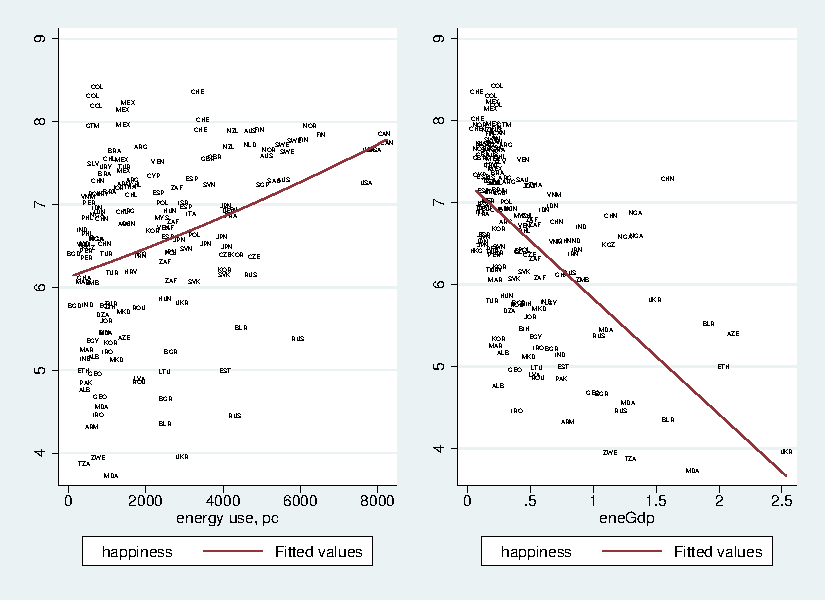
\includegraphics[height=3in]{graphsAndTables/couWvsGrComEneGdp.pdf}\centering
\caption{couWvsGrComEneGdp}\label{couWvsGrComEneGdp}
\end{figure}
{\scriptsize Note: Country codes are in table \ref{ls} in supplementary
  material. If country was observed in more than one year, the data were averaged.}

latin american ctries like COL or MEX very little energy per gdp; while post
soviet like ukraine or MDA BLR AZE ARM are very energy intesive and miserable

What is striking is the differences in energy use by area. Diferences are
severalfold. Mexico and Colombia
consume only ??? and yet are as happy as ??? which consumes ???.

\begin{figure}[H]
 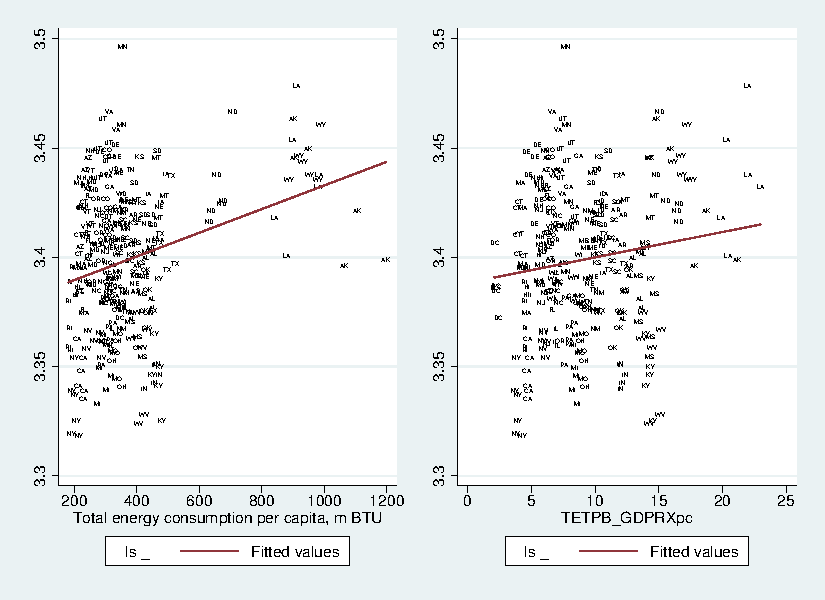
\includegraphics[height=3in]{graphsAndTables/grComTETPB_gdp.pdf}\centering
\caption{grComTETPBgdp}\label{grComTETPBgdp}
\end{figure}
{\scriptsize TODO Note: Country codes are in table \ref{ls} in supplementary
  material. If country was observed in more than one year, the data were averaged.}

for states teh positive results are divern only by LA, ND, WY, AK; othersie
nothing there, can do a graph dropping those

\begin{figure}[H]
 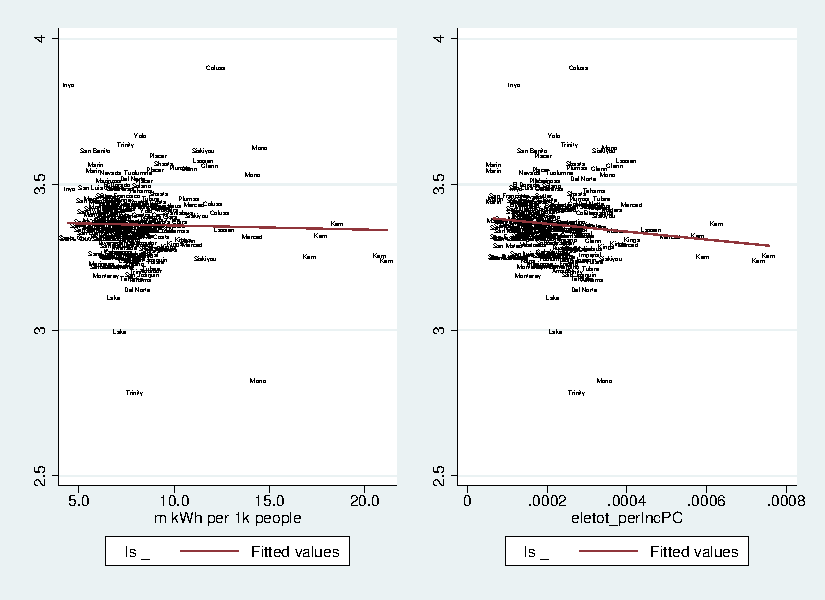
\includegraphics[height=3in]{graphsAndTables/eletot_gdp.pdf}\centering
\caption{eletotgdp}\label{eletotgdp}
\end{figure}
{\scriptsize Note: Country codes are in table \ref{ls} in supplementary
  material. If country was observed in more than one year, the data were averaged.}

%note: cen div is somewhat weird...


so need to have more gdp, less energy use, at least across countries...


What is striking is the differences in energy use by area. Diferences are
severalfold. Mexico and Colombia
consume only ??? and yet are as happy as ??? which consumes ???.


\begin{figure}[H]
 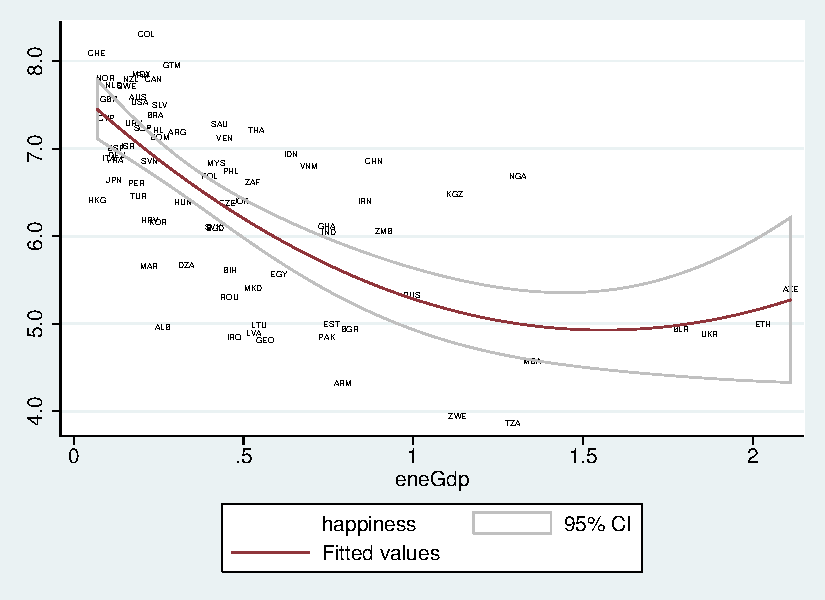
\includegraphics[height=3in]{graphsAndTables/couWvsLsEnePerGdp.pdf}\centering
\caption{total energy use divided by gdp}\label{}
\end{figure}
{\scriptsize TODO Note: Country codes are in table \ref{ls} in supplementary
  material. If country was observed in more than one year, the data were averaged.}

\begin{figure}[H]
 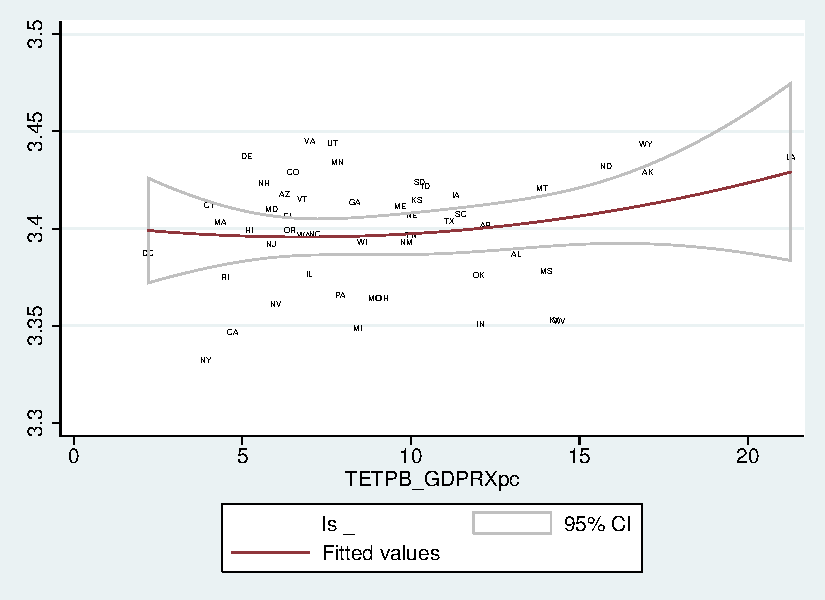
\includegraphics[height=3in]{graphsAndTables/lfTETPBgdpLS.pdf}\centering
\caption{total energy use divided by gdp}\label{}
\end{figure}
{\scriptsize TODO Note: state codes are in table \ref{ls} in supplementary
  material. If country was observed in more than one year, the data were averaged.}

\begin{figure}[H]
 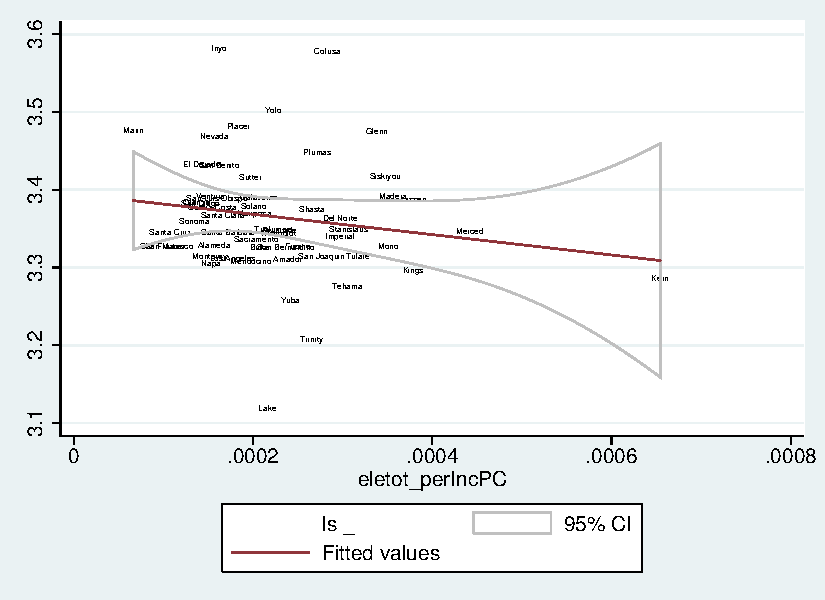
\includegraphics[height=3in]{graphsAndTables/caEleTotGdp.pdf}\centering
\caption{total energy use divided by gdp}\label{}
\end{figure}
{\scriptsize TODO Note: Country codes are in table \ref{ls} in supplementary
  material. If country was observed in more than one year, the data were averaged.}

\begin{figure}[H]
 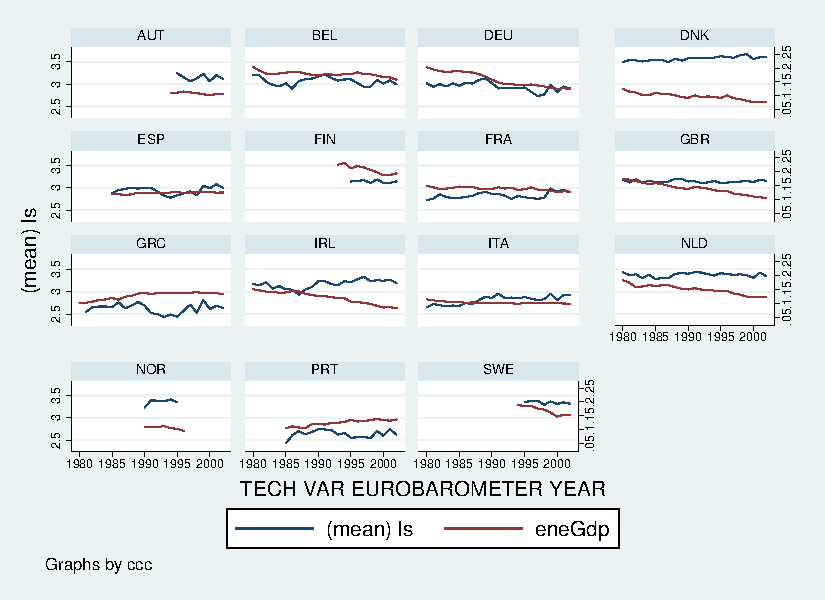
\includegraphics[height=3in]{graphsAndTables/ebTSeneGdp.pdf}\centering
\caption{happiness and (total) energy intesity of gdp}\label{ebTSeneGdp}
\end{figure}

\begin{figure}[H]
 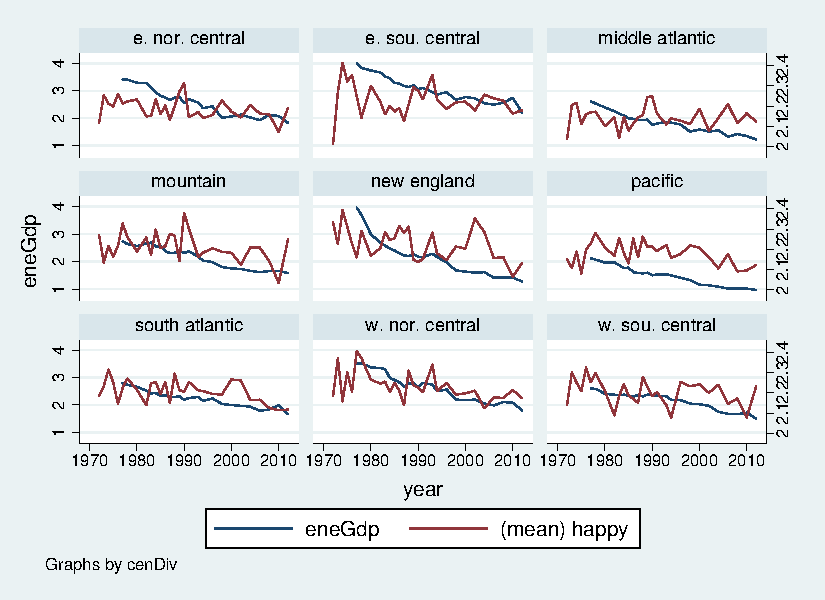
\includegraphics[height=3in]{graphsAndTables/cenDiveneGdp.pdf}\centering
\caption{happiness and (residential) energy intesity of gdp}\label{cenDiveneGdp}
\end{figure}

maybe this approach in gigures \ref{cenDiveneLs} and \ref{ebTSeneLs} is a way to
go--we have energy intesity of gdp so maybe do energy intesity of happiness!
especially that Sen recently adocated to use happiness to measure progress.

\begin{figure}[H]
 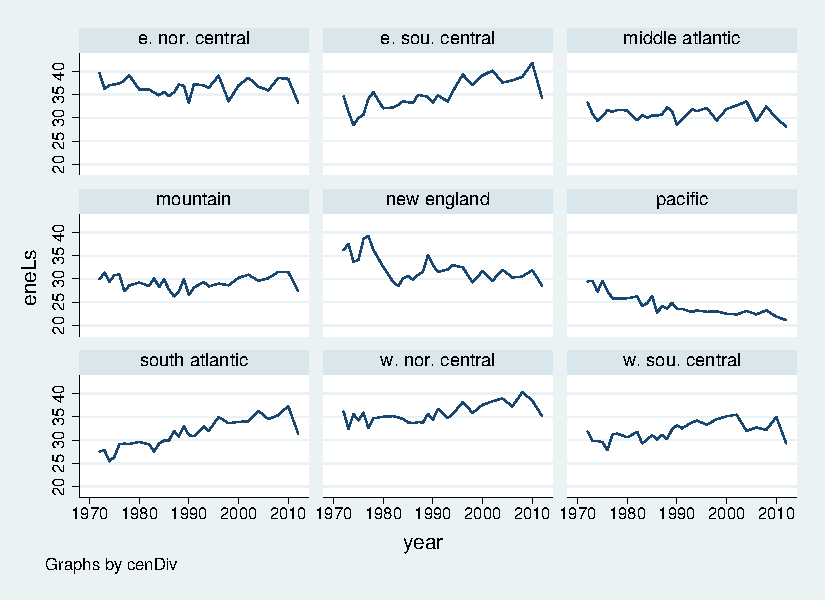
\includegraphics[height=3in]{graphsAndTables/cenDiveneLs.pdf}\centering
\caption{happiness and (residential) energy intesity of happiness--Pacific is
  doing great--maybe Green California? While East is considerably worse! }\label{cenDiveneLs}
\end{figure}

\begin{figure}[H]
 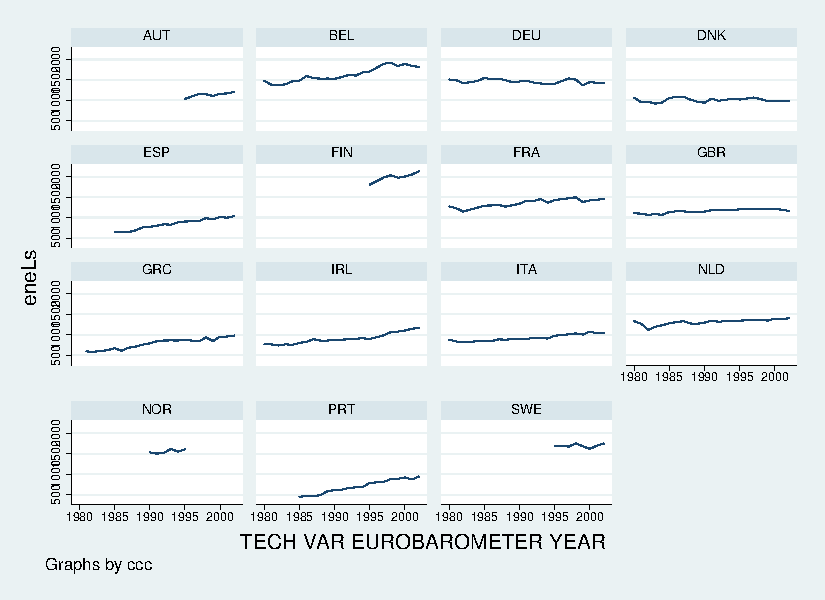
\includegraphics[height=3in]{graphsAndTables/ebTSeneLs.pdf}\centering
\caption{Europe is getting worst and worst; Northern Scandinavian countries
  worse--arguably because it is cold tehre, while Southern are lower}\label{ebTSeneLs}
\end{figure}

\subsection{multivariate: other things}
\label{mvarOthThings}

So how come there is not much in bivariate relationship except in the
World--well as already hinted at in that first figure, there are other things
going on, like GDP that we controlled for in that figure, adn so we would
explore some of those things here. At the same time, this section sets the stage
for the future research and explores a bit some of those ideas.
\textbf{TODO:} can discuss here some loiterature as i guess i had it earlier at
the beginning in tghe literature review and then removed to that other pdf file...


And we also take into accouint more factors in the regressions framework in the
online appendix

\begin{figure}[H]
 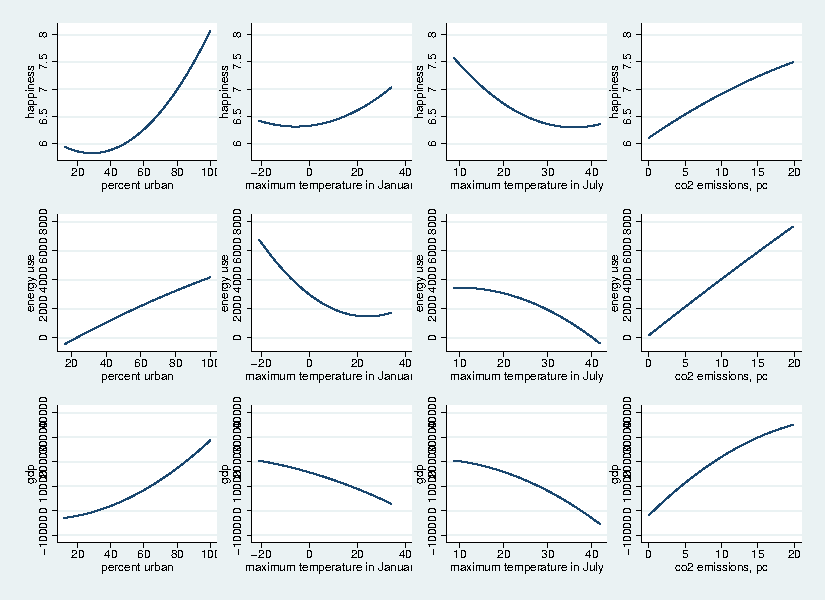
\includegraphics[width=6in]{graphsAndTables/mat1.pdf}\centering
\caption{id: mat1;  note that this is total energy, not residential, and it is not avergaed
over yrs}\label{mat1}
 \end{figure}


\subsubsection{multivariate: other things:: but gasoline consumption is good !}

well, driving may be result of happiness: happy people go places; miserable
folks stay home and watch tv; and may reflect overall mood of the
place--activity or even business cycle i guess

\begin{figure}[H]
 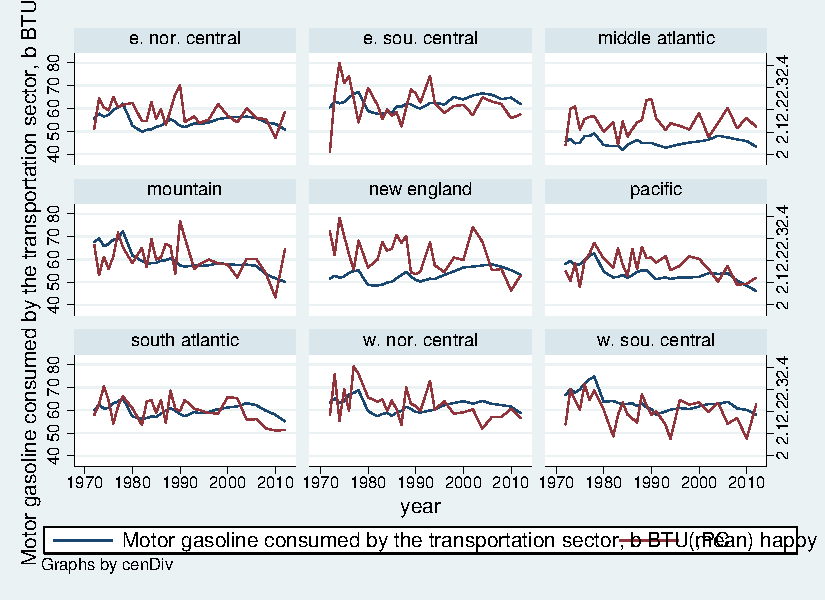
\includegraphics[width=6in]{graphsAndTables/cenDivLsYrMGAPB.pdf}\centering
\caption{but driving is good !}\label{cenDivLsYrMGAPB}
 \end{figure}

\subsubsection{multivariate: other things:: but natural gas consumption is good !}

\begin{figure}[H]
 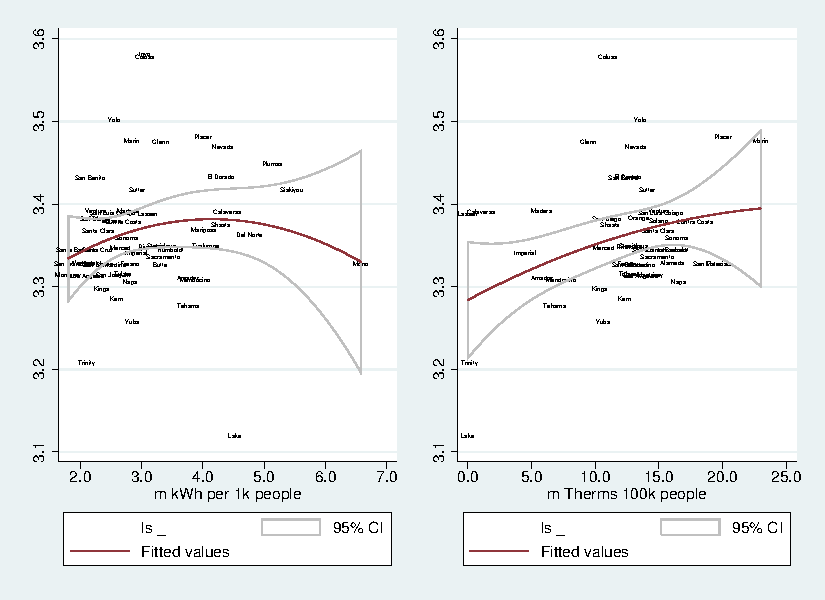
\includegraphics[width=6in]{graphsAndTables/caEleGas.pdf}\centering
\caption{driving is good in california as well ! (left electrisity; right gas)}\label{cenDivLsYrMGAPB}
 \end{figure}

\subsubsection{multivariate: other things:: breaking it down by other things: hi--lo}

\begin{figure}[H]
 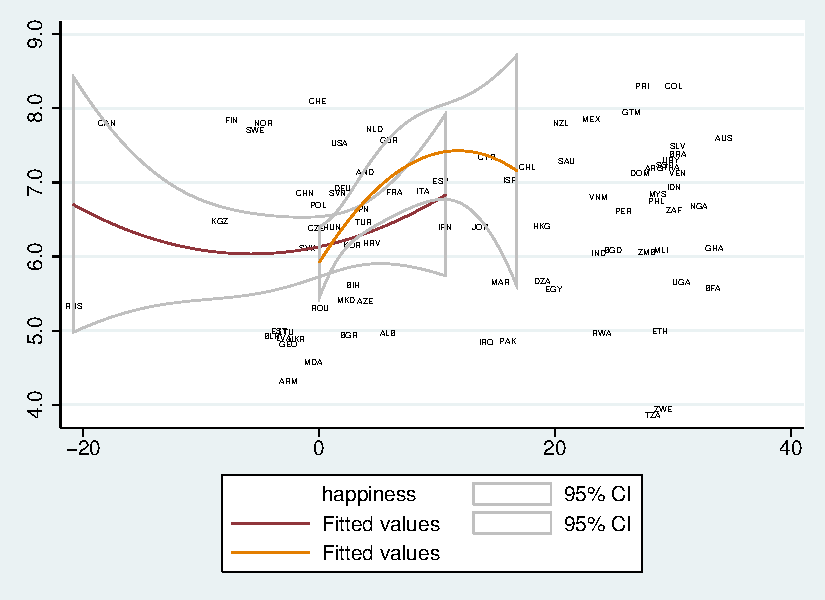
\includegraphics[width=6in]{graphsAndTables/co2twice.pdf}\centering
\caption{}\label{cenDivLsYrMGAPB}
 \end{figure}

\begin{figure}[H]
 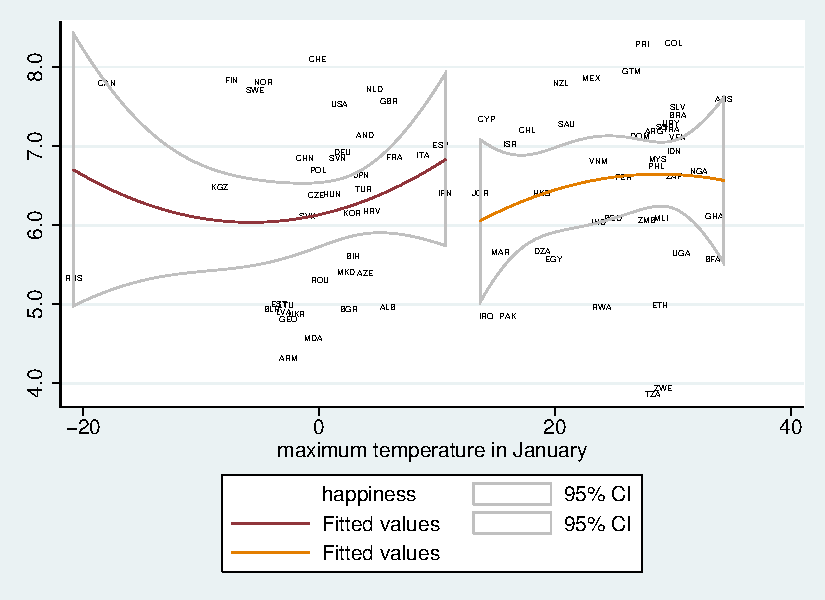
\includegraphics[width=6in]{graphsAndTables/JanTwice.pdf}\centering
\caption{}\label{JanTwice}
 \end{figure}

\begin{figure}[H]
 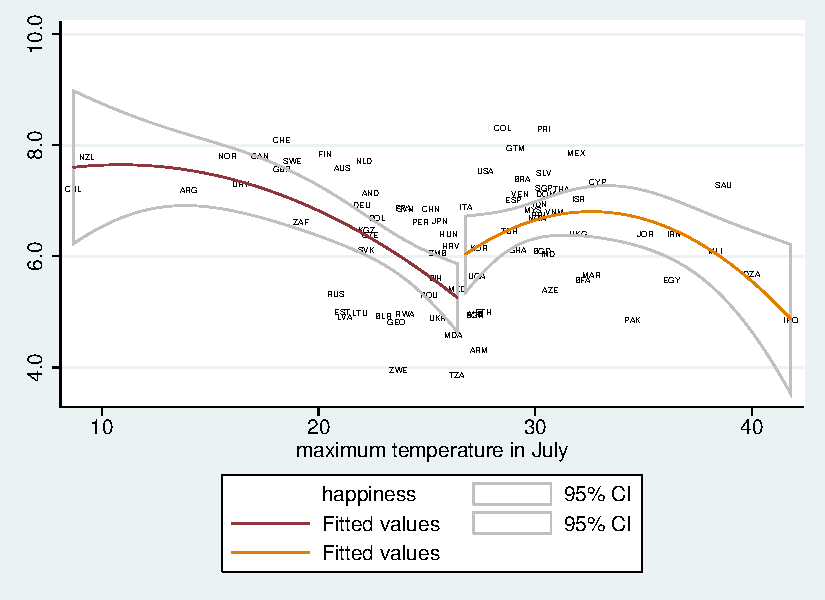
\includegraphics[width=6in]{graphsAndTables/JulTwice.pdf}\centering
\caption{}\label{JulTwice}
 \end{figure}

\begin{figure}[H]
 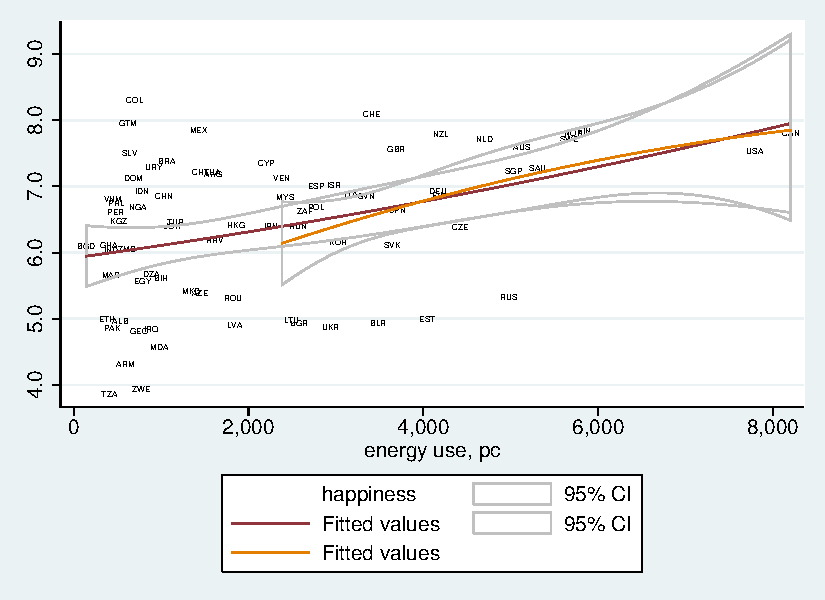
\includegraphics[width=6in]{graphsAndTables/eneTwice.pdf}\centering
\caption{}\label{eneTwice}
 \end{figure}



\section{Theoretical/conceptual additional information}

\subsection{What Do We Know So Far? The Literature}

% Micah -- We shouldn't set out to write a literature review. (No one should, except as part of a student thesis). The point is to put our findings in appropriate context. 
% Rely on the literature to establish 3 things:
% - the significance of the broad problem -- which should be supported by cites in the intro
% - that the problem being solved in the paper is important and hasn't been solved
% - that the rationale for the methods applied is sound

Energy use is getting more efficient due to technological imporvements and the
world economy is growing and hence every year we use less energy per gdp, but
still both energy use and co2 emissions, which correlate at above 90 percent,
are still growing every year \cite{iea14}. 


It is striking then that large happiness literature has omitted topic of energy
so far--threre are no studies about energy consumption and happiness across
areas, and only one study across persons.  \cite{graef81} (recently republished
as \cite{csikszentmihalyi14}) is the  only study about energy consumption and
happiness. This was a person-level study that used experience
sampling method (ESM) and it found no relationship between energy consumption
and happiness or even a negative relationship for females. 

% Micah: Few are stricken by the literature. What is striking is the universal assumption that
% consumption makes people happy, and the lack of any convincing empirical exampination of this claim.

Going back to initial question of how to achieve both happiness and
sustainabilty--we are not the first to try to answer it, we are only to fist to
do it using happiness and energy measures. Others used other measures.
Literature does look at the effect of energy consumption on human
wellbeing, but operationalizes human wellbeing differently--mostly as HDI or its
components. And literature proposes various indices linking HDI or its
components to natural resources or environment.

For instance, \cite{dietz09} proposed environmentally efficient wellbeing
(EWEB) as function of economic, natural and human resources. A simlar, but
closer to energy focus of present study is \cite{jorgenson14B} who proposed
energy intensity of human wellbeing. Yet, again, all of these approaches remain
in the realm of HDI or its components, GDP, education and life expectancy. 
 Using human development index (HDI) \cite{steinberger10} and argues along the
 same lines as present paper: increasing energy consumption beyond a point does
 not contribute anymore to wellbeing.  Many more studies link enrgy use to HDI
 \cite[e.g.]{dias06}, yet HDI, like  GDP, has its limitations--for an overview
 see \cite{klugman11}--and hence  recently happiness was proposed as another
 measure of broadly understood human  development--incidentally Amartya Sen both
 co-introduced HDI in 1990 and  reently advocatdes happiness \cite{stiglitz09al}. 

We will use happiness measure. But it is worth noting that there is also
 happy years measure (happiness$*$life expectancy) \cite{veenhoven96B}, and
 finally Happy Planet Index ($\frac{happiness*life\;expectancy}{ecological\;footprint}$)--this is somewaht close approach to  ours, except that we will try to see how energy consuption specifically afects  happiness. And there are few more: Genuine Progress Indicator, Ecological Footprints,  and planetary boundaries--see p. 477 in \cite{pretty13} for  sources. 

% Micah: The three paragraphs above are organized backward. State what we're doing first, then why we chose to do it, and what it adds to scientific knowledge. Don't ignore other work, but be positive.

While there is no literature about energy use and happiness, there is related
literature. \cite{pretty13} provides a wonderful overview of the relationship
betweenresource consumption, economy and wellbing including happiness measure of
it. There is literature about relationship between happiness and outcomes
related to energy consumption or attitudes about consumption. First, pollution makes us unhappy \cite{weinhold12,welsch05}. Second,
and more important,  there is some evidence that happy people
are more sustainable, that is, happiness affects sustainability
\cite{ericson14}.  Causation possibly goes in the
other direction as well (as noted by authors), but in general it is
safe to say that happiness and sustainable behavior are correlated  \cite{brown05,corral11}.

Then there is energy efficiency that moderaters (or mediates?) the relationship
between energy use and happiness--it is not only that energy use that results in
happiness, but importantly its efficient use--one country may waste lots of
energy say due to outdated and inefficent technologies as those in 1990s in
Eastern Europe, whereas some other ountry can actually use less energy per
capita but actually deliver more wellebing because enrgey is better used. We
will accounty for  energy efficiency by controlling for  $CO_2$ emissions. 
 A country that can produce more energy with less $CO_2$ is more energy
 efficient--perhaps a crude measure but readily available for a large sample of
 countries. There are better measures (e.g. \url{http://www.aceee.org/research-report/e1402}) but available for only a handful of countries
%can
                                %also do co2 per gdp  guess also can do co2 per
                                %energy etc etc

A related issue is that of ``rebound problem'' or the Jevons paradox
\cite{pretty13}%p476-477
--efficiency frees up resources that are then used to increase consumption, and
hence technological progress or efficient technology by itself does not lead to
sustainability. While in the developed World, energy consumption is flat or even
decreasing, it is globally increasing due to the developing World
\cite{pretty13}. Energy consumption, like economic growth and consmption has no
limit--indeed, instead of satysfying our needs it stimulates them--''the more
one has the more one wants, since satisfactions received only stimulate instead
of filling needs''   \cite{durkheim50}. This brings us to three major happiness
theories, all relevant to this study. 

% The three paragraphs above don't belong here. The appropriate time to introduce this information is to integrate it into the approach or discussion of interventions, to the extent this prior work is important for  what we should choose to measure, or for the design of appropriate interventions.



Before answering a question of how is happiness created, let's define it first. 
  Happiness, or the more scientific term Subjective Well-Being (SWB), is ``both cognitive judgments of one's life
satisfaction in addition to affective evaluations of mood and
emotions'' \cite[p. 142]{steel08},  or in other words: ``overall judgment of life that draws on two sources of information:
  cognitive comparison with standards of the good life (contentment) and
  affective information from how one feels most of the time (hedonic
  level of affect).''(\cite[p. 2]{veenhoven08})
 Some scholars make a
  distinction between happiness and life satisfaction--life
  satisfaction refers to cognition and happiness refers to affect. In practice,
  however, it is usually difficult  if not impossible to separate the two
  concepts.  Hence, the overall happiness definition by 
   \cite{veenhoven08}, as quoted above,  seems most appropriate and we will use terms
   ``happiness,''``life satisfaction'' and ``(subjective) wellbeing'' interchangeably.  For a recent and very through statement of
happiness measure validity and reliability see \cite{diener09}
(especially ch. 5). 

% Micah: Explain why this is the best way of defining happiness for the purposes of understanding energy consumption.
There are many ways to measure human wellbeing. Traditionally, we have used
income measures such as per capita gross dometic product or health measures such
as life exectancy or human development measures such as education. %HDI index 
 It has been recognized recently, however, that these measures do not capture
 human wellbeing well--two key problems are that these measures are not
 comprehensive enough and it is difficult to combine them into a single measure
 because weights are always arbitrary. The co-inventor of the original
 development metric (Human Development Index), Amartya Sen, has recently
 proposed happiness as a better measure \cite{stiglitz09al}.

\subsection{The three happiness theories}
The adaptation theory \cite{brickman78cj} argues that there is
adjustment to external circumstances and we are on a 'hedonic
treadmill.' ``The more one has the more one wants, since satisfactions
received only stimulate instead of filling needs''\cite{durkheim50}. 
We arguably get used to (adapt to) energy consumption, too. Hence, increasing
energy consumption is futile for our happiness, because we will adapt to it and
always want more.
%
The  multiple discrepancy theory  \cite{michalos85} states that
happiness is a result of social comparison or a comparison to various
standards.  I compare my consumption to others. I also compare
it to standards--for instance, that of people in my geographic or social
proximity. Notably, this may result in consumption arms race--people wanting to
outcompete others in terms of consumption in a vicious
cycle \cite{frank12}. Hence, also like  per adaptation theory, energy consumtion
will not result in geater happiness.  
%
  The needs/livability theory \cite{veenhoven95, veenhoven14b} posits that
  happiness results from objective living conditions and from
  fulfillment of our needs, and predicts that higher physical or economic
  development will result in greater happiness. It is not clear, however, if
  there is any limit to the level of development that should result in greater
  happiness as it is not clear what is the limit to human needs. Of course, one
  could argue that there are needs and wants, and while there are some clearly
  defined needs (e.g. biological), most other needs are relative and
  subjective. Hence, based on this theory, as opposed to the other two theories,
  greater energy use will result in greater happiness.
  
\subsection{Future Research}

TODO set research agenda somewhare!! for future research!

There are many ideas for future research. Indeed, as mentioned earlier, one of
the goals of this study is to encourage more research on this important and
overlooked topic of energy consumption and happiness.

We just examined total energy use per capita at country level without
differentiating between sectors, because we could not find ssuch data. There are
however enrgy use data by sector for smaller sets of countries--for instance for
Europe available from Eurostat: 
\url{http://epp.eurostat.ec.europa.eu/portal/page/portal/energy/data/database}, \url{http://epp.eurostat.ec.europa.eu/portal/page/portal/energy/data/main_tables} 

We suggest that clean energy would result in greater happiness. This idea could
poissibly be tested more direcly by examining happiness of people in areas where
clean energy is prevalent. 


Yet, energy efficiency or even clean energy is not the final solution due to
``rebound problem'' or the Jevons paradox--due to innate human greed we are
likely to consume ever more and more, and hence the only lasting solution is to
curb our energy hunger possibly through public policy and education.


\subsection{Comparability of Results}

We did not make same scales on graphs for reason of interpretaility. We could
make both scales, happiness and energy standarized, but then it is more
difficult to intepret results, we think. In this approach, we have followed
\cite{easterlin10B,easterlin12}, who also used different unstandarized
happiness scales in the same study. 



\section{What is Wrong With Texas?}

There are obviously many things wrong with Texas, but we would like to focus on
consumption, energy use, eceonomic development in general and envrionment. They
say that ``everything is big in Texas,'' 

This paper was born on the Sprit\footnote{Author is a social scientist and
  cannot afford non-frugal airlines.} flight 215 approaching DFW airport. I am
flying PHL-DFW every month and always wonder about energy use when I approach
Dallas. From the airplane you see big roads and huge highways connecting bi
houses (so called McMansions) with huge shopping areas. And you see big cars and
in them big Texans (Texans are not big enough yet to spot them from the
airplane, but you'll see them once you land). I though rom he airplane, geez,
they must use twice as much energy as on east coats, and checked data adn bingo
! they do about 2x (TODO gve exact numbers). 
Texas economy is growing fast but its open land is shrinking fast, too--and you
can see that from the airpplane, too--there is a sea of concrete as far as eye
can see; and there is some fake nauture constantly tended by Mexicans who use
more energy to cut grass and sweep with those air blowers. But numbers say the
same--Texas lost about 1.1 million acres between 1997 and 2012. 
\cite{marshallCL14}


\section{General Considerations}

\subsection{Electricty use: residential and non-residential} 
How is electricity used in United States homes? This is an important
consideration because it really shows what we do with this electricity--how we
consume it, what are the end uses. Data are shown in table
\ref{eleEndUse}. Furthermore end uses of energy changed over time, for instance
 from 1993 to 2009: applianes share increased from 24\% to 35\% and space
 heating dropped from 53\% to 41\%
 \url{http://www.eia.gov/todayinenergy/detail.cfm?id=10271&src=%E2%80%B9%20Consumption%20%20%20%20%20%20Residential%20Energy%20Consumption%20Survey%20%28RECS%29-b1}. 
Also, the good news is that average energy consumption per household dropped from 114 m BTU in 1980 to
90 m BTU in 2009 \url{http://www.eia.gov/consumption/residential/reports/2009/consumption-down.cfm?src=%E2%80%B9%20Consumption%20%20%20%20%20%20Residential%20Energy%20Consumption%20Survey%20%28RECS%29-b5}.  


\begin{table}[H]\centering\footnotesize
\caption{\label{eleEndUse}  Estimated U.S. Residential Electricity Consumption by End
  Use, 2012 \url{www.eia.gov/tools/faqs/faq.cfm?id=96&t=3}}
\begin{tabular} {llll}   \hline 
End Use&Quadrillion\\\hline 
Btu &Billion\\
kilowatthours &Share of\\
total \\
Space cooling&0.85&250&18.00\%\\
Lighting&0.64&186&14.00\%\\
Water heating&0.45&130&9.00\%\\
Refrigeration&0.38&111&8.00\%\\
Televisions and related equipment 1&0.33&98&7.00\%\\
Space heating&0.29&84&6.00\%\\
Clothes dryers&0.2&59&4.00\%\\
Computers and related equipment2&0.12&37&3.00\%\\
Cooking&0.11&31&2.00\%\\
Dishwashers3 &0.1&29&2.00\%\\
Furnace fans and boiler circulation pumps&0.09&28&2.00\%\\
Freezers&0.08&24&2.00\%\\
Clothes washers3&0.03&9&1.00\%\\
Other uses4&1.02&299&22.00\%\\
Total consumption&4.69&1375&\\\hline
\end{tabular}\end{table}


\subsection{TODO Petroleum use: residential and non-residential} 
\subsection{TODO Natural Gas use: residential and non-residential} 

\section{countries}

Literature about happiness across countries usually focuses on role of income,
with a well known Easterlin Paradox, where economic growth does not lead to
greater happiness over time.\footnote{veenhoven's criticsim--have it
somewhere--easterlin delusion etc}. Yet, in space, across countries it is agreed
upon that richer countries are happier at least with quadratic relationship. 

In this study we aregue that countries that consumer more enrgy are not happier
when controlling for income--and interpret this as another argument for energy
conservation. Also it counters commoin wisodom--one could think that greater
energy consumption leasd to greater happiness--if not then whatt;s the point of
energy consumption. 

One explanation is that sustainable people are happy (cite that i think
ecological economics paper--shoudl be in ebib)


\subsection{europe-mannheim}

\begin{figure}[H]
 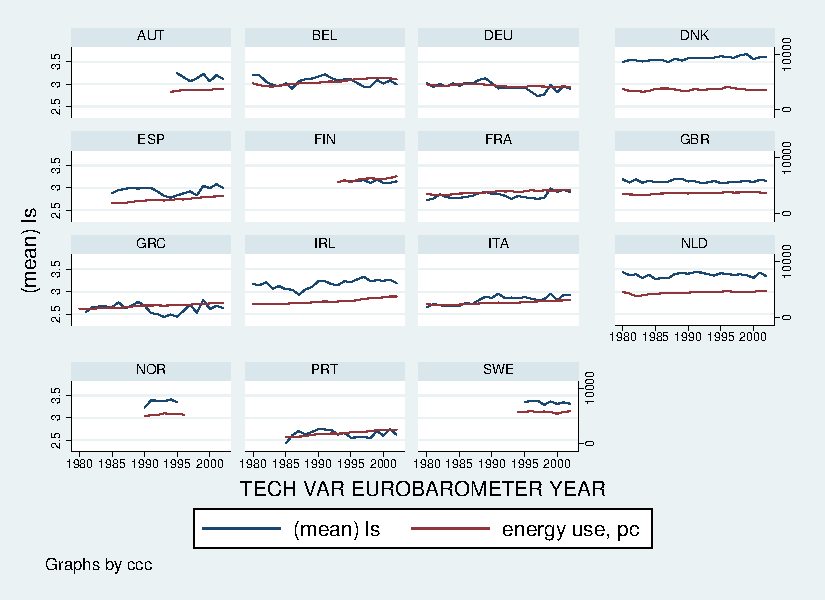
\includegraphics[width=6in]{graphsAndTables/ebTS.pdf}\centering
\caption{and over time not much relationship either !yet somehow corr is actually .5 }\label{ebTS}
\end{figure}


\ig{graphsAndTables/couLsEne.pdf}

\ig{graphsAndTables/couLsGdp.pdf}

\subsection{world}

\ig{graphsAndTables/couWvsLsEne.pdf}

\ig{graphsAndTables/couWvsLsGdp.pdf}

very interesting--when controlling fpr gdp, energy becomes negativbe!!
\ig{graphsAndTables/couWvsLsEnGdp.pdf}



\section{Census Divisions}

\begin{figure}[H]
 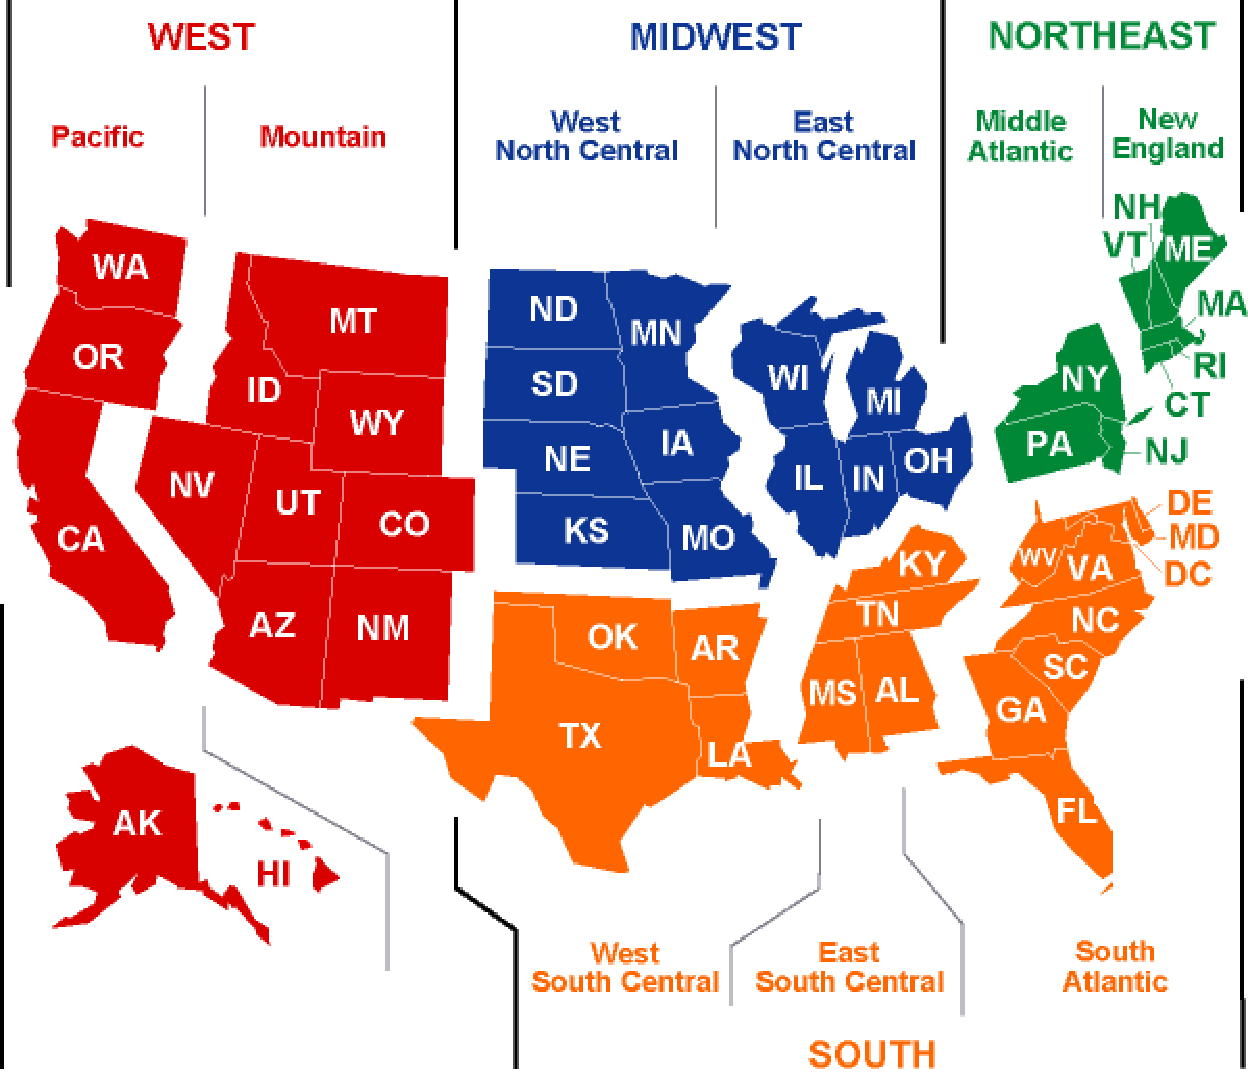
\includegraphics[height=3in]{graphsAndTables/cendivco.pdf}\centering
\caption{Census divisions.}\label{cenDiv}
\end{figure}

have a ts graph here showing happiness by division and lectricity
consumption--guess smooth them

\section{States}

This paper started as one author frequently flies from NJ to TX and noticed from
the air and on the ground huge differences in energy use between the two
states. Bigger houses, roads, cars, indeed everything is big in Texas! And
indeed differences are striking--Texas consumee about twice as much enbrgy as NJ
does per capita; yet interestingly not a big difference in residential energy
consumption--perhaps everything is newer in TX and hence more enrgy
efficent. The biggest diffences are in transportation ?? v ?? --


\begin{spacing}{.8}
{\footnotesize
\begin{verbatim}
TETPB    Total energy consumption per capita, m BTU
TERPB    Total energy consumption per capita in the residential sector, m BTU
TEAPB    Total energy consumption per capita in the transportation sector, m BTU
TECPB    Total energy consumption per capita in the commercial sector, m BTU
TEIPB    Total energy consumption per capita in the industrial sector, m BTU

sorted on TETPB, this is for 2009

. | state   TETPB   TERPB   TEAPB   TECPB   TEIPB |
  |-----------------------------------------------|
  |    RI     182      58      60      44      20 |
  |    NY     192      56      56      62      18 |
  |    HI     205      27     100      31      48 |
  |    MA     211      65      69      42      35 |
  |    CA     212      40      84      41      47 |
  |-----------------------------------------------|
  |    CT     215      71      68      52      23 |
  |    AZ     219      59      76      52      31 |
  |    FL     222      66      77      54      25 |
  |    NH     227      69      80      51      27 |
  |    NV     244      58      80      43      63 |
  |-----------------------------------------------|
  |    VT     248      80      85      47      36 |
  |    MD     256      74      81      74      27 |
  |    OR     269      68      87      51      63 |
  |    NC     273      78      76      63      56 |
  |    NJ     273      68     103      72      31 |
  |-----------------------------------------------|
  |    MI     274      76      75      61      62 |
  |    UT     274      59      86      55      74 |
  |    PA     287      73      77      54      83 |
  |    DE     294      77      79      71      67 |
  |    CO     296      68      85      60      83 |
  |-----------------------------------------------|
  |    IL     303      76      78      63      86 |
  |    GA     304      76      98      57      73 |
  |    WA     307      77      91      59      80 |
  |    VA     308      81      93      78      56 |
  |    ME     311      68      94      48     101 |
  |-----------------------------------------------|
  |    WI     313      76      76      63      98 |
  |    MO     313      89      96      69      59 |
  |    OH     321      81      82      61      98 |
  |    DC     324      61      34     222       7 |
  |    NM     325      57      99      59     110 |
  |-----------------------------------------------|
  |    ID     326      82      80      55     109 |
  |    TN     333      84      96      60      93 |
  |    MN     340      77      90      66     108 |
  |    SC     345      79      99      57     110 |
  |    AR     360      78     100      57     125 |
  |-----------------------------------------------|
  |    MS     379      75     122      54     128 |
  |    WV     382      94      92      60     136 |
  |    AL     384      78      98      54     153 |
  |    KS     402      84     102      75     141 |
  |    OK     403      80     121      65     137 |
  |-----------------------------------------------|
  |    IN     423      87      92      59     186 |
  |    NE     431      88      99      77     168 |
  |    MT     431      90     116      81     144 |
  |    KY     449      89     110      60     191 |
  |    TX     452      64     110      58     219 |
  |-----------------------------------------------|
  |    SD     453      90     113      77     173 |
  |    IA     477      81     100      68     227 |
  |    ND     656     103     133      98     321 |
  |    LA     841      79     150      62     550 |
  |    AK     904      77     273      89     465 |
  |-----------------------------------------------|
  |    WY     933      85     217     111     519 |
  +-----------------------------------------------+

(obs=306)

             |    TERPB    TEAPB    TECPB    TEIPB    TETPB
-------------+---------------------------------------------
       TERPB |   1.0000
       TEAPB |   0.2141   1.0000
       TECPB |   0.2132   0.1255   1.0000
       TEIPB |   0.3914   0.7993   0.1818   1.0000
       TETPB |   0.4418   0.8620   0.3274   0.9757   1.0000


(obs=306)

             |    TERPB    TEAPB    TECPB    TEIPB    TETPB       ls
-------------+------------------------------------------------------
       TERPB |   1.0000
       TEAPB |   0.2141   1.0000
       TECPB |   0.2132   0.1255   1.0000
       TEIPB |   0.3914   0.7993   0.1818   1.0000
       TETPB |   0.4418   0.8620   0.3274   0.9757   1.0000
          ls |   0.0952   0.2740   0.1246   0.2629   0.2839   1.0000

ls is happiness
\end{verbatim}
}
\end{spacing}

Furthermore, interestingly transportation corrlates negatively with commerce--DC
one of the most effiicnet in trasportation (61) is least efficient in commerce
(222).  Total energy consumption correlates most with transportation (.86) and
 especially industry (.9). Happiness does correlate positively with all energy
 uses, mostly with transport and industry and total (about .3). 
  

\begin{figure}[H]
 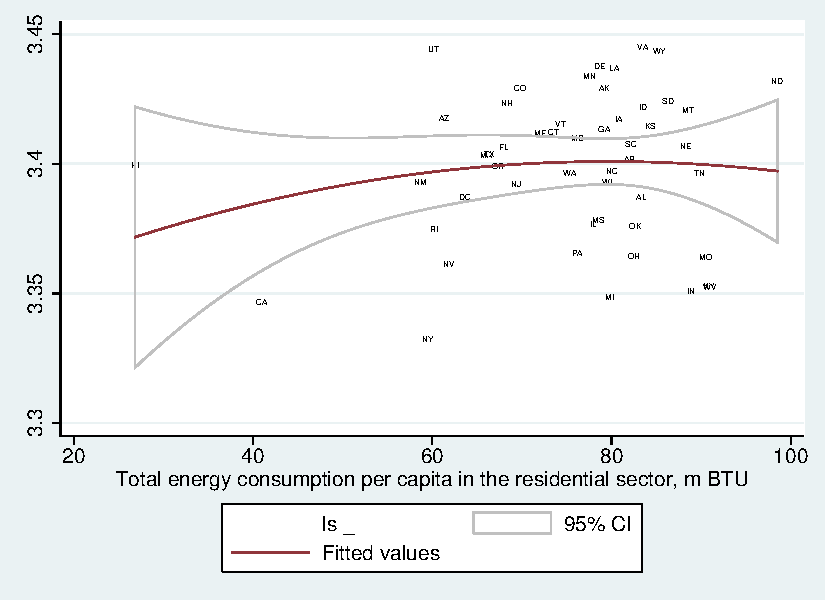
\includegraphics[height=3in]{graphsAndTables/lfTERPBls.pdf}\centering
\caption{lfTERPBls}\label{lfTERPBls}
\end{figure}

\begin{figure}[H]
 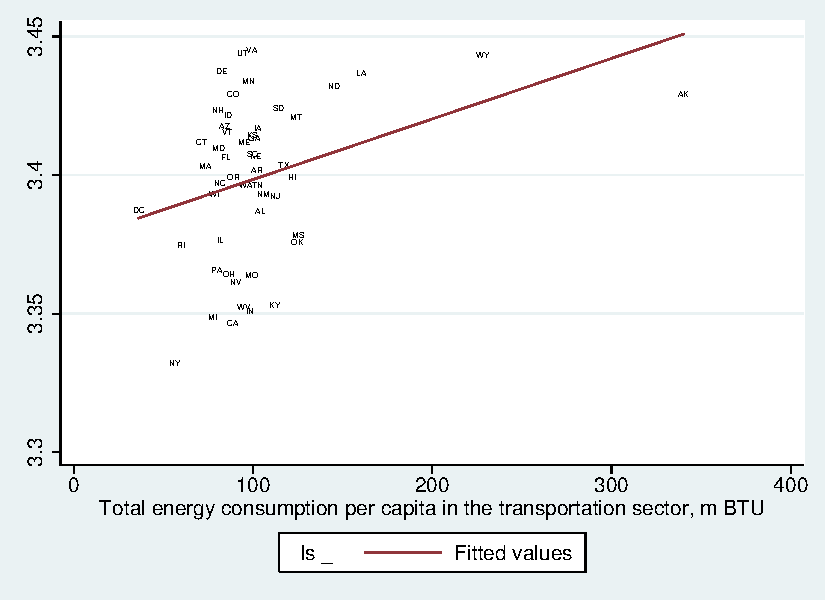
\includegraphics[height=3in]{graphsAndTables/lfTEAPBls.pdf}\centering
\caption{lfTEAPBls}\label{lfTEAPBls}
\end{figure}

\begin{figure}[H]
 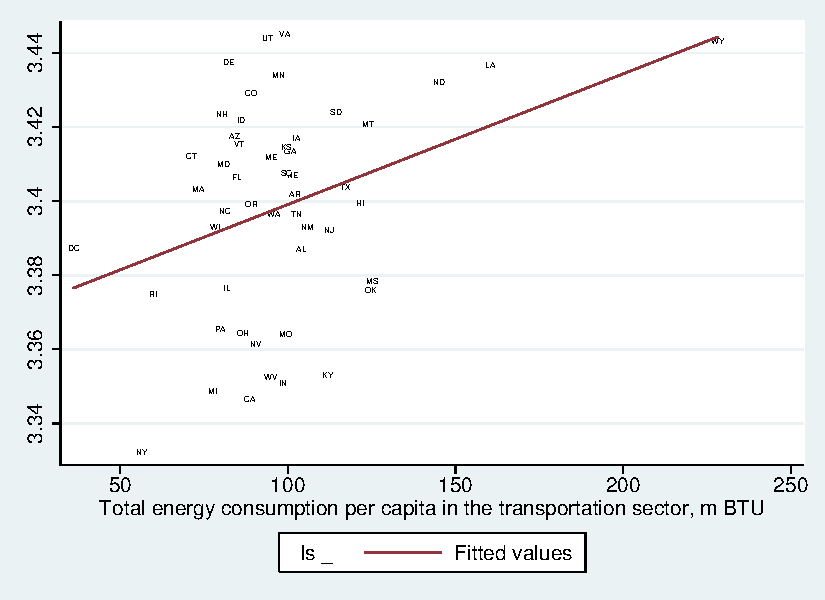
\includegraphics[height=3in]{graphsAndTables/lfTEAPBlsNoAk.pdf}\centering
\caption{no alaska; lfTEAPBlsNoAk}\label{lfTEAPBlsNoAk}
\end{figure}

\begin{figure}[H]
 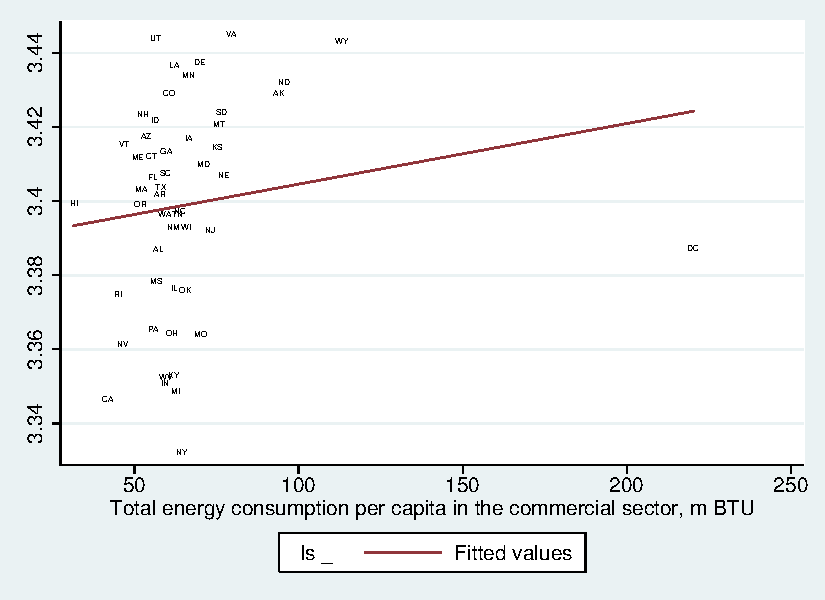
\includegraphics[height=3in]{graphsAndTables/lfTECPBls.pdf}\centering
\caption{lfTECPBls}\label{lfTECPBls}
\end{figure}

\begin{figure}[H]
 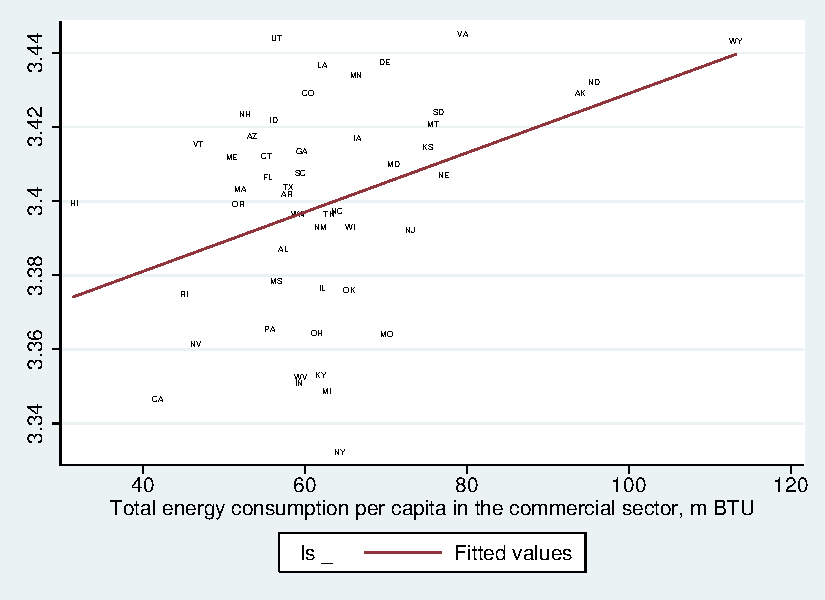
\includegraphics[height=3in]{graphsAndTables/lfTECPBlsNoDc.pdf}\centering
\caption{lfTECPBlsNoDc}\label{lfTECPBlsNoDc}
\end{figure}

\begin{figure}[H]
 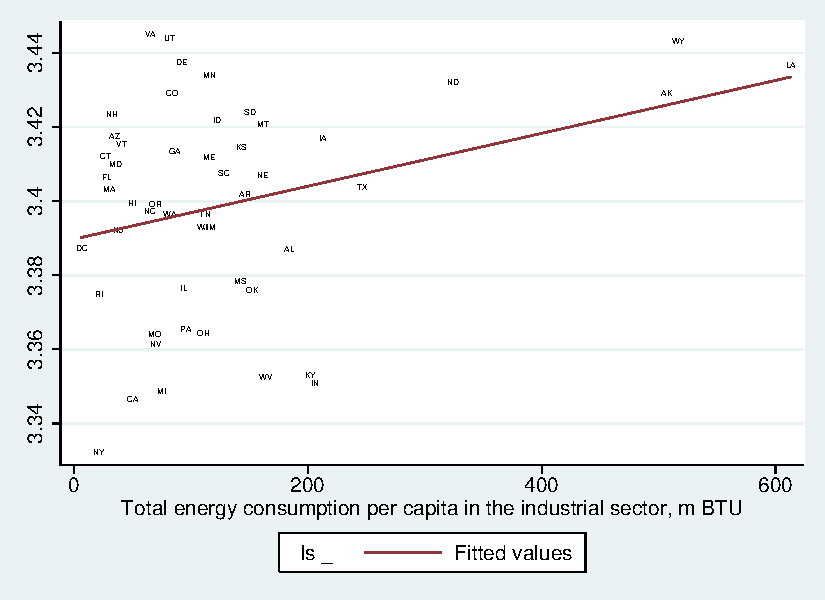
\includegraphics[height=3in]{graphsAndTables/lfTEIPBls.pdf}\centering
\caption{lfTEIPBls}\label{lfTEIPBls}
\end{figure}

\begin{figure}[H]
 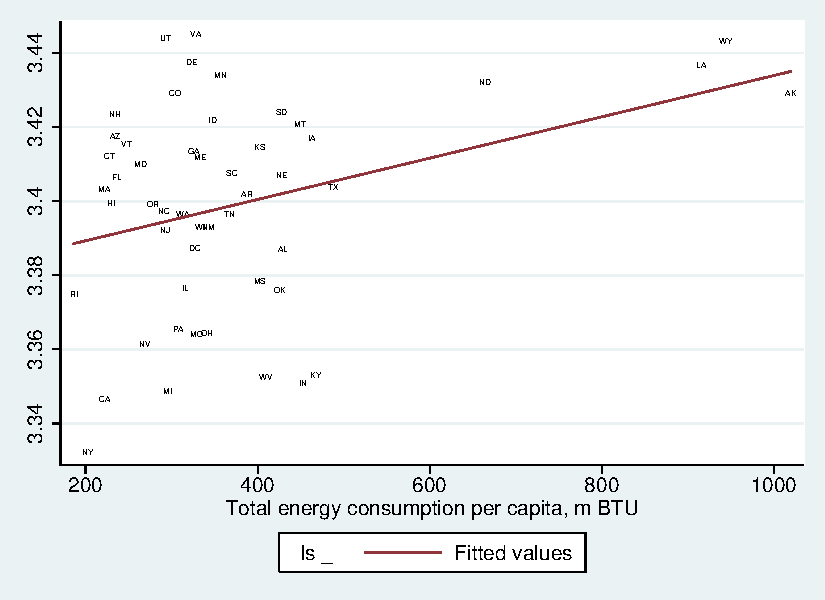
\includegraphics[height=3in]{graphsAndTables/lfTETPBls.pdf}\centering
\caption{lfTETPBls}\label{lfTETPBls}
\end{figure}


 We 
expect the  more dense and more urban areas are less happy. Note that ppulation
density and percent urban are very different variables--population density is
largely driven by history-when state was established--Western States (except
California) are less dense than North Eestern states. It is also driven by  size
of state--large states like Pennsylvania are less dense than smaller states like
Rhode Island. Percent urban is different--and it reflects administrative
prcesses such as zoning and is sensitive to a defninition of urban area. There are large differences in both
variables. In some North Eastern states there are more than 1,000 people per
square mile (NJ, RI), in most Western states, on the other hand, there are fewer
than 100 people per square mile. Several states are above 90\% urban, yet few
states are mostly non urban. Below a table sorted on population density.

Finally, we will look at 2 key variables for happiness, social support, one
measure of social capital, and the other ``harder'' measure--general
health. States in West and North are more supportive with an exception of
Delaware, which is very supportive and surrounded by unsupportive states.


\begin{spacing}{.8}
\begin{verbatim}
  | state     popDen   perUrb |  .  +---------------------+ 
  |---------------------------|     | state   supp     gh | 
  |    AK   .0012512    66.02 |     |---------------------| 
  |    WY   .0058089    64.76 |     |    HI   4.03   3.52 | 
  |    MT   .0068089    55.89 |     |    NY   4.05   3.60 | 
  |    ND    .009768     59.9 |     |    CA   4.09   3.53 | 
  |    SD   .0107636    56.65 |     |    DC   4.10   3.72 | 
  |---------------------------|     |    TX   4.11   3.46 | 
  |    NM   .0170242    77.43 |     |---------------------| 
  |    ID   .0190094    70.58 |     |    MS   4.11   3.30 | 
  |    NE   .0238206    73.13 |     |    AZ   4.13   3.57 | 
  |    NV   .0246217     94.2 |     |    CT   4.15   3.71 | 
  |    UT   .0337594    90.58 |     |    PA   4.15   3.55 | 
  |---------------------------|     |    FL   4.16   3.52 | 
  |    KS   .0349687     74.2 |     |---------------------| 
  |    OR   .0399737    81.03 |     |    MI   4.17   3.53 | 
  |    ME   .0430245    38.66 |     |    SC   4.18   3.47 | 
  |    CO   .0487062    86.15 |     |    NV   4.18   3.51 | 
  |    IA   .0546036    64.02 |     |    RI   4.19   3.64 | 
  |---------------------------|     |    IN   4.19   3.48 | 
  |    OK      .0548    66.24 |     |---------------------| 
  |    AR    .056154    56.16 |     |    KY   4.20   3.35 | 
  |    AZ   .0564202    89.81 |     |    MO   4.20   3.48 | 
  |    MS   .0632948    49.35 |     |    NM   4.21   3.51 | 
  |    MN   .0666861    73.27 |     |    AR   4.21   3.42 | 
  |---------------------------|     |    MT   4.21   3.59 | 
  |    VT   .0679205     38.9 |     |---------------------| 
  |    WV   .0771272    48.72 |     |    OH   4.21   3.51 | 
  |    MO   .0872253    70.44 |     |    IL   4.21   3.53 | 
  |    AL   .0945003    59.04 |     |    NE   4.22   3.61 | 
  |    TX   .0966383     84.7 |     |    AL   4.22   3.34 | 
  |---------------------------|     |    NH   4.22   3.69 | 
  |    WA   .1014513    84.05 |     |---------------------| 
  |    WI   .1050449    70.15 |     |    NJ   4.22   3.61 | 
  |    LA   .1051988    73.19 |     |    OR   4.23   3.58 | 
  |    KY    .110114    58.38 |     |    CO   4.23   3.69 | 
  |    NH   .1471073     60.3 |     |    NC   4.23   3.47 | 
  |---------------------------|     |    WA   4.24   3.59 | 
  |    TN   .1541655    66.39 |     |---------------------| 
  |    SC   .1542213    66.33 |     |    ME   4.24   3.60 | 
  |    GA   .1688821    75.07 |     |    SD   4.25   3.64 | 
  |    MI   .1746762    74.57 |     |    VT   4.25   3.74 | 
  |    IN   .1811528    72.44 |     |    ID   4.25   3.57 | 
  |---------------------------|     |    OK   4.25   3.38 | 
  |    NC   .1966354    66.09 |     |---------------------| 
  |    VA   .2031902    75.45 |     |    MA   4.26   3.74 | 
  |    HI   .2123741    91.93 |     |    MD   4.26   3.63 | 
  |    IL   .2312725    88.49 |     |    VA   4.27   3.63 | 
  |    CA   .2396597    94.95 |     |    LA   4.27   3.40 | 
  |---------------------------|     |    WY   4.27   3.63 | 
  |    OH   .2825454    77.92 |     |---------------------| 
  |    PA   .2840687    78.66 |     |    KS   4.27   3.60 | 
  |    FL   .3514421    91.16 |     |    GA   4.28   3.54 | 
  |    NY   .4116164    87.87 |     |    WI   4.28   3.61 | 
  |    DE   .4618843     83.3 |     |    AK   4.28   3.64 | 
  |---------------------------|     |    UT   4.29   3.71 | 
  |    MD    .596153     87.2 |     |---------------------| 
  |    CT   .7391024    87.99 |     |    IA   4.29   3.60 | 
  |    MA   .8414038    91.97 |     |    ND   4.30   3.59 | 
  |    RI   1.018562    90.73 |     |    WV   4.30   3.26 | 
  |    NJ      1.197    94.68 |     |    MN   4.31   3.72 | 
  |---------------------------|     |    DE   4.31   3.62 | 
  |    DC          .      100 |     |---------------------| 
  +---------------------------+     |    TN   4.32   3.42 | 
\end{verbatim}                      +---------------------+ 
\end{spacing}


Below regressions follow.  We have
seen that there is a weak to modearte relationshipe between energy use per
capita in different sectors and in general and happiness. How do these
relationships hold in regrressions? We proceed in a following way. We look at
three major energy uses: residential, commericial ,and transport  and also
total. We leave off indusrtial hence this energy is less liekly to impact
werllbeing of people directly and it may bias it--because this energy use is
dicatted by industry--there may be indiorect effects--thourgh employment, wages
adn development, but that shoudl be picked up by GDP. 
First, we
consider a model where we control for level of economic development (per capita
incoime). Then we add envioronmental factors, density, percent urban and avergae
temoertaures in Jan and Jul follwoning \cite{abdallah08al, brereton08}--we use
average for each month Jun and Jul and not the single max day. Finally, and this
is perhaps innovation in ecological literature, we add at state level two
aggregated from BRFSS key person level prodictors of happiness--social support
and happiness--tehre is substantail variation on these variables as discussed earlier.

We do not control for crime that is distributed unevenly within each state, and
hence global control in not informative.  

Let's start with residential energy, TERPB.
In column 1, relationship is positive  However, once controlling in column 2 for
population density and percent urban and tempoeratures , the relationship
between TERPB and happiness disappears. Likewise, when added in column 3
controls for social support and general health, the raltionship stays
non-existent. 


In transportation (TEAPB), on the other hand, the relationship is
positive, and if anything it increases with added controls, which is
puzzling. There are at least 2 explanations--perhaps thrill of travel %TODO cite
                                %from my ls_car paper  
Also, Americans prefer \cite{fuguitt90,fuguitt75} and are happier
\cite{aok_hea_spr,aok11a} in suburbs than in big cities, and there are likely
to be more consumption of energyu  in ransportatin in states woith more suburbs.
Likewise, when considering total energy use (TETPB) a positive relationship
persists. This warrants further exploration. 

\begin{table}[H]\centering \caption{ols1} \label{ols1} \begin{scriptsize} \begin{tabular}{p{1.4in}p{.43in}p{.43in}p{.43in}p{.43in}p{.43in}p{.43in}p{.43in}p{.43in}p{.43in}p{.43 in}p{.43in}p{.43 in}}\hline                     &      TERPB1   &      TERPB2   &      TERPB3   &      TEAPB1   &      TEAPB2   &      TEAPB3   &      TETPB1   &      TETPB2   &      TETPB3   \\
Total energy consumption per capita in the residential sector, m BTU&       0.000+  &       0.000   &       0.000   &               &               &               &               &               &               \\
Total energy consumption per capita in the transportation sector, m BTU&               &               &               &       0.000***&       0.000** &       0.000***&               &               &               \\
Total energy consumption per capita, m BTU&               &               &               &               &               &               &       0.000***&       0.000+  &       0.000***\\
Real gross domestic product, m chain 05usd, PC&       0.000+  &       0.002***&       0.001***&       0.000*  &       0.002***&       0.000+  &       0.000   &       0.002***&       0.000   \\
popukation density, thosands per sq m&               &      -0.029***&      -0.023***&               &      -0.022** &      -0.012** &               &      -0.024** &      -0.012*  \\
perUrb              &               &      -0.001***&      -0.001***&               &      -0.000** &      -0.000***&               &      -0.001** &      -0.000***\\
avgJanTemp          &               &      -0.000   &       0.001***&               &      -0.000   &       0.001***&               &      -0.000   &       0.001***\\
avgJulTemp          &               &       0.001*  &       0.002***&               &       0.001*  &       0.002***&               &       0.001*  &       0.002***\\
gh                 &               &               &       0.204***&               &               &       0.221***&               &               &       0.233***\\
supp               &               &               &       0.203***&               &               &       0.201***&               &               &       0.191***\\
constant            &       3.368***&       3.261***&       1.654***&       3.369***&       3.256***&       1.605***&       3.373***&       3.263***&       1.616***\\
N                   &         306   &         288   &         288   &         306   &         288   &         288   &         306   &         288   &         288   \\
 \hline\multicolumn{6}{l}{+p$<$0.10 *p$<$0.05 **p$<$0.01 ***p$<$0.001; robust standard errors} \end{tabular}\end{scriptsize}\end{table}


First considering enrgy use in residential and in commerce (columns a),
interestingly it appears that the positive relationship is driven by commerce,
residential energyu use indeed  turns negative. Then in columns b, when
considering all, three, residential, commerce, and transportation, thw first two
remain insignificant and transportation coomes out positive


\begin{table}[H]\centering \caption{ols2} \label{ols2} \begin{scriptsize} \begin{tabular}{p{1.4in}p{.43in}p{.43in}p{.43in}p{.43in}p{.43in}p{.43in}p{.43in}p{.43in}p{.43in}p{.43 in}p{.43in}p{.43 in}}\hline                     &          a1   &          a2   &          a3   &          b1   &          b2   &          b3   \\
Total energy consumption per capita in the residential sector, m BTU&       0.000   &      -0.000   &      -0.000+  &       0.000   &      -0.000   &      -0.000   \\
Total energy consumption per capita in the transportation sector, m BTU&               &               &               &       0.000***&       0.000   &       0.000***\\
TET*                &               &               &               &               &               &               \\
Total energy consumption per capita in the commercial sector, m BTU&       0.000   &       0.001***&       0.001***&      -0.000   &       0.000   &      -0.000   \\
Real gross domestic product, m chain 05usd, PC&       0.000   &       0.002***&       0.000*  &       0.000   &       0.002***&       0.000+  \\
popukation density, thosands per sq m&               &      -0.023** &      -0.018***&               &      -0.022** &      -0.012** \\
perUrb              &               &      -0.001***&      -0.001***&               &      -0.001** &      -0.000** \\
avgJanTemp          &               &      -0.000   &       0.001***&               &      -0.000   &       0.001***\\
avgJulTemp          &               &       0.001*  &       0.002***&               &       0.001*  &       0.002***\\
gh                 &               &               &       0.201***&               &               &       0.218***\\
supp               &               &               &       0.208***&               &               &       0.204***\\
constant            &       3.374***&       3.280***&       1.665***&       3.350***&       3.276***&       1.603***\\
N                   &         306   &         288   &         288   &         306   &         288   &         288   \\
 \hline\multicolumn{6}{l}{+p$<$0.10 *p$<$0.05 **p$<$0.01 ***p$<$0.001; robust standard errors} \end{tabular}\end{scriptsize}\end{table}

These findings are lagrly replicated with fixed effects estimatiion--there is no
increase in happiness from energy use in residential or total, but tehre is an
increase in transportation. Note, hausman test indicates that we should use
fixed, not random effect.  


\begin{table}[H]\centering \caption{fe1} \label{fe1} \begin{scriptsize} \begin{tabular}{p{1.4in}p{.43in}p{.43in}p{.43in}p{.43in}p{.43in}p{.43in}p{.43in}p{.43in}p{.43in}p{.43 in}p{.43in}p{.43 in}}\hline                     &      TERPB1   &      TERPB2   &      TERPB3   &      TEAPB1   &      TEAPB2   &      TEAPB3   &      TETPB1   &      TETPB2   &      TETPB3   \\
Total energy consumption per capita in the residential sector, m BTU&      -0.001+  &      -0.001   &      -0.000   &               &               &               &               &               &               \\
Total energy consumption per capita in the transportation sector, m BTU&               &               &               &      -0.000+  &      -0.000   &       0.000+  &               &               &               \\
Total energy consumption per capita, m BTU&               &               &               &               &               &               &      -0.000   &       0.000   &       0.000   \\
Real gross domestic product, m chain 05usd, PC&       0.003***&       0.003***&       0.003***&       0.003***&       0.003** &       0.002** &       0.003***&       0.002*  &       0.002** \\
popukation density, thosands per sq m&               &       0.456   &       0.027   &               &       0.532   &       0.175   &               &       0.687+  &       0.135   \\
perUrb              &               &       0.011***&       0.008** &               &       0.011***&       0.008** &               &       0.011***&       0.008** \\
avgJanTemp          &               &       0.000   &       0.000   &               &       0.000+  &       0.000   &               &       0.001*  &       0.000   \\
avgJulTemp          &               &       0.003***&       0.002***&               &       0.002***&       0.001** &               &       0.002***&       0.002***\\
gh                 &               &               &       0.212***&               &               &       0.220***&               &               &       0.212***\\
supp               &               &               &       0.162***&               &               &       0.168***&               &               &       0.161***\\
constant            &       3.307***&       2.211***&       1.168***&       3.288***&       2.193***&       1.033***&       3.285***&       2.140***&       1.134***\\
N                   &         306   &         288   &         288   &         306   &         288   &         288   &         306   &         288   &         288   \\
 \hline\multicolumn{6}{l}{+p$<$0.10 *p$<$0.05 **p$<$0.01 ***p$<$0.001; robust standard errors} \end{tabular}\end{scriptsize}\end{table}


%TODO defineitly have beta coeff some hwere--see what ecological econ
%doeas--maybe in app if they don;t do that a lot..


\subsection{More state-level graphs}

\begin{figure}[H]
 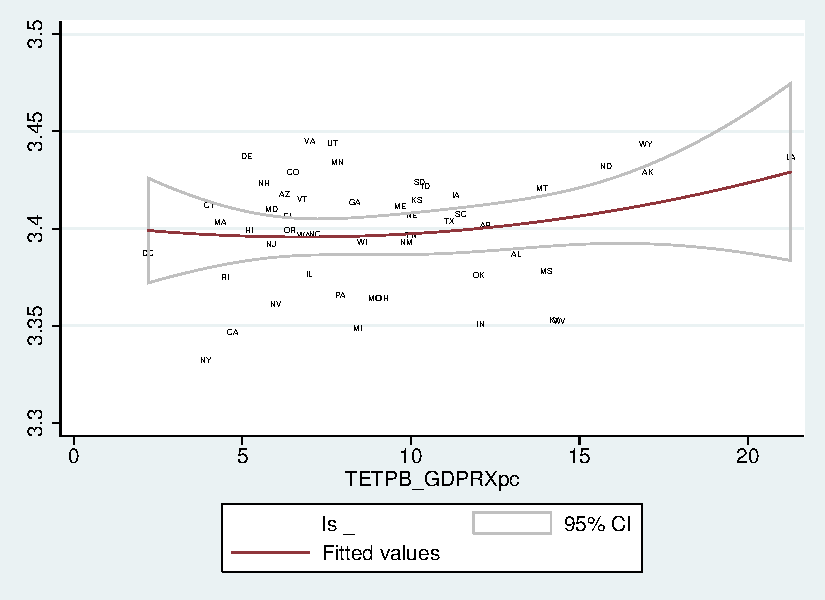
\includegraphics[width=6in]{graphsAndTables/lfTETPBgdpLS.pdf}\centering
\caption{Not much relationship here--note the scale of happiness--very small
  differences and much of that driven by WY, AK, and LA.}\label{lfTETPBgdpLS}
\end{figure}


\section{Counties}

\begin{figure}[H]
 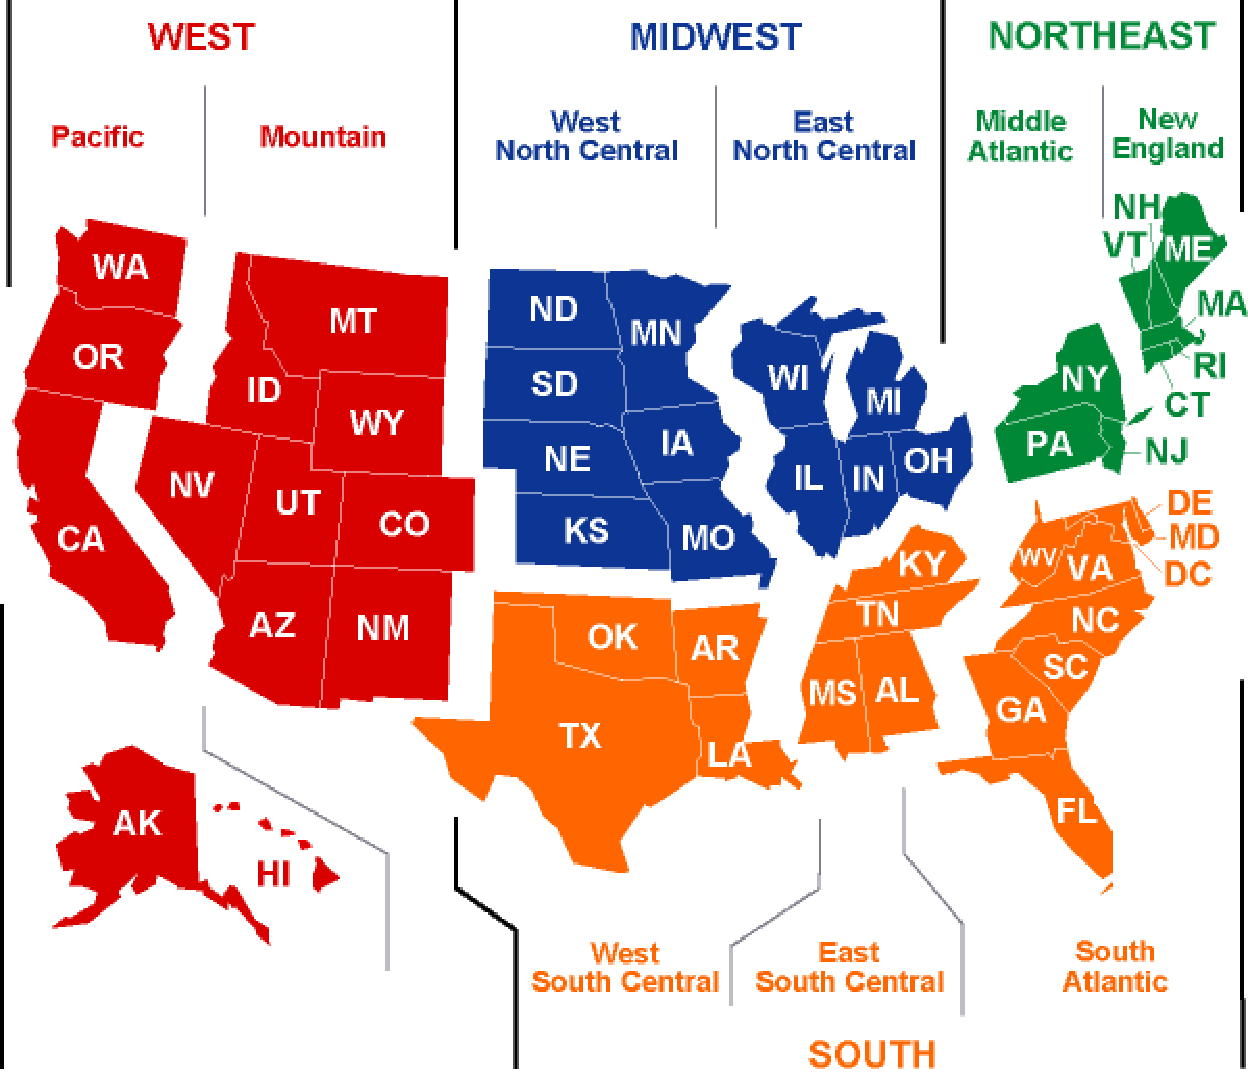
\includegraphics[height=3in]{graphsAndTables/cendivco.pdf}\centering
\caption{California climate divisions correspondencies with California
  counties. \url{http://www.cpc.ncep.noaa.gov/products/analysis_monitoring/regional_monitoring/CLIM_DIVS/california.gif}.}\label{caCD}
\end{figure}

Note, as shown in figure \ref{caCD}, there is not always an exact overlap
between counties and climate divisions. They were matched in the following way

The limitation of states is that, well, it is very ecological--large areas! and
second, there is not much difference is happijess ascross states, buit there is
much more across counties. 

Here in bivariate case, too, like across states, there is a positive
relationshipe between energy consumprion and happiness, yet it is somewhat
weaker. 

\begin{figure}[H]
 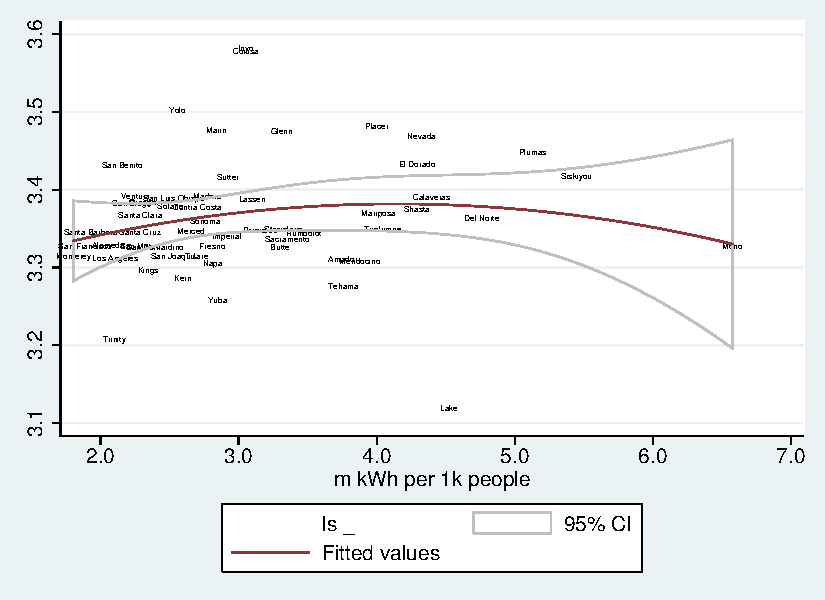
\includegraphics[height=3in]{graphsAndTables/lfELERESls.pdf}\centering
\caption{lfELERESls}\label{lfELERESls}
\end{figure}

\begin{figure}[H]
 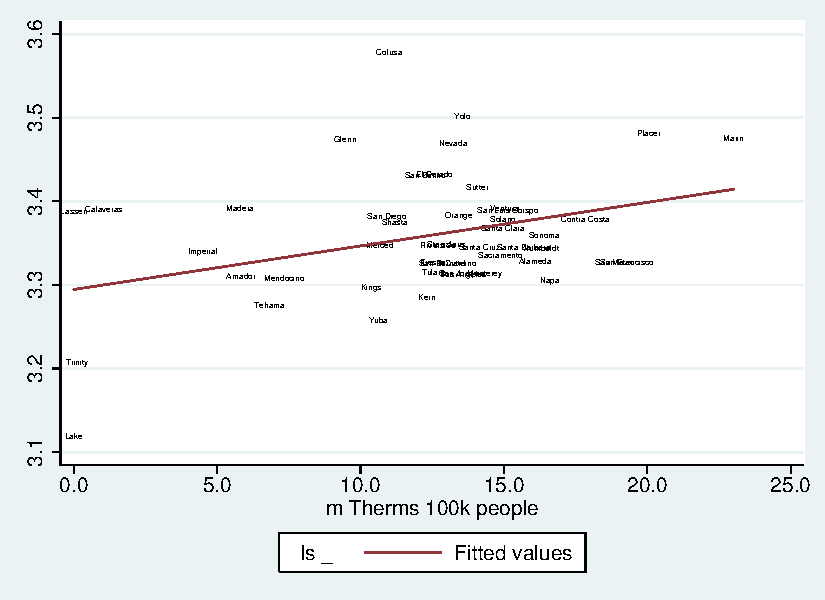
\includegraphics[height=3in]{graphsAndTables/lfGASls.pdf}\centering
\caption{lfGASls}\label{lfGASls}
\end{figure}



\begin{spacing}{.8}
\begin{verbatim}
SORTED OON ELERES
  ----------------------------------+
           county   eleres   eletot |
  ----------------------------------|
          Trinity      0.8      8.1 |
         Monterey      1.8      5.9 |
             Inyo      1.9      4.5 |
    Santa Barbara      1.9      7.5 |
    San Francisco      1.9      7.3 |
  ----------------------------------|
      Los Angeles      2.0      6.8 |
          Alameda      2.0      7.2 |
       San Benito      2.1      5.6 |
        San Diego      2.1      6.1 |
          Ventura      2.1      6.5 |
  ----------------------------------|
      Santa Clara      2.2      9.3 |
   San Bernardino      2.2      6.5 |
        San Mateo      2.3      6.6 |
            Kings      2.3      9.7 |
           Orange      2.3      6.9 |
  ----------------------------------|
       Santa Cruz      2.3      4.8 |
           Solano      2.4      7.5 |
  San Luis Obispo      2.4      6.1 |
      San Joaquin      2.4      8.1 |
             Yolo      2.5      8.2 |
  ----------------------------------|
             Kern      2.5     17.7 |
           Tulare      2.5      8.5 |
           Merced      2.6     14.1 |
     Contra Costa      2.6      8.8 |
           Madera      2.7      9.1 |
  ----------------------------------|
           Fresno      2.7      7.5 |
             Napa      2.8      7.5 |
            Marin      2.8      5.6 |
           Sonoma      2.8      5.9 |
           Sutter      2.8      6.3 |
  ----------------------------------|
             Yuba      2.8      6.7 |
        Riverside      2.8      6.2 |
         Imperial      2.8      8.0 |
           Colusa      3.0     12.0 |
           Lassen      3.0     11.5 |
  ----------------------------------|
       Stanislaus      3.2      8.9 |
       Sacramento      3.2      7.5 |
            Glenn      3.3     10.7 |
            Butte      3.3      6.5 |
         Humboldt      3.6      6.8 |
  ----------------------------------|
           Tehama      3.7      7.8 |
           Amador      3.7      8.4 |
           Placer      3.8      8.4 |
        Mendocino      3.9      6.8 |
         Mariposa      4.0      6.2 |
  ----------------------------------|
         Tuolumne      4.1      8.1 |
           Shasta      4.2      8.8 |
        El Dorado      4.2      6.9 |
           Nevada      4.3      6.7 |
        Calaveras      4.4      7.1 |
  ----------------------------------|
             Lake      4.6      7.0 |
        Del Norte      4.8      8.1 |
           Plumas      5.2     10.2 |
         Siskiyou      5.4     11.2 |
             Mono      6.6     14.5 |
  ----------------------------------|
           Alpine        .        . |
           Sierra        .        . |
            Modoc        .        . |
  				   
  ----------------------------------+

SORTED ON GASRES

           county   gasres   gastot |
  ----------------------------------|
             Lake      0.0      0.0 |
           Lassen      0.0      0.0 |
          Trinity      0.2      0.5 |
        Calaveras      1.0      2.0 |
         Imperial      4.4     17.6 |
  ----------------------------------|
           Madera      5.8     28.3 |
           Amador      5.8     24.1 |
           Tehama      6.9     17.3 |
        Mendocino      7.3     12.1 |
            Glenn      9.5     27.6 |
  ----------------------------------|
            Kings     10.2     44.9 |
           Merced     10.6     45.3 |
             Yuba     10.7     16.6 |
        San Diego     10.9     18.1 |
           Colusa     11.1    121.9 |
  ----------------------------------|
           Shasta     11.4     19.2 |
        Riverside     12.1     18.3 |
             Kern     12.1    276.3 |
       San Benito     12.2     23.7 |
           Fresno     12.3     30.3 |
  ----------------------------------|
           Tulare     12.4     35.3 |
        El Dorado     12.7     17.3 |
       Stanislaus     12.9     33.6 |
   San Bernardino     13.2     24.1 |
           Orange     13.4     21.2 |
  ----------------------------------|
           Nevada     13.4     19.1 |
            Butte     13.4     21.6 |
             Yolo     13.5     30.9 |
      San Joaquin     13.5     28.9 |
           Sutter     13.8     22.7 |
  ----------------------------------|
      Los Angeles     13.8     31.8 |
         Monterey     13.9     26.0 |
       Santa Cruz     13.9     21.9 |
      Santa Clara     14.5     25.6 |
       Sacramento     14.8     22.2 |
  ----------------------------------|
          Ventura     14.9     24.3 |
  San Luis Obispo     15.0     29.3 |
           Solano     15.1     54.6 |
    Santa Barbara     15.5     29.9 |
         Humboldt     15.7     24.7 |
  ----------------------------------|
          Alameda     15.8     27.7 |
           Sonoma     16.0     23.7 |
             Napa     16.6     29.2 |
           Placer     17.6     26.1 |
     Contra Costa     17.8     96.4 |
  ----------------------------------|
        San Mateo     18.4     30.7 |
    San Francisco     19.0     32.7 |
            Marin     22.6     31.4 |
            Modoc        .        . |
           Alpine        .        . |
  ----------------------------------|
        Del Norte        .        . |
         Siskiyou        .        . |
             Inyo        .        . |
           Plumas        .        . |
             Mono        .        . |
  ----------------------------------|
           Sierra        .        . |
         Mariposa        .        . |
         Tuolumne        .        . |
  ----------------------------------+

\end{verbatim}
\end{spacing}


And now regressions. Natural gas usage is a function of its availabily, not
necassarily gas hunger--for instance Lassen County has zero natural gas
use. Furthermore if gas is unused then it may be compensated with other sources,
hence electricty and gas in one regression. And as expected, no effect in
happiness. 

\begin{table}[H]\centering \caption{CAols1} \label{CAols1} \begin{scriptsize} \begin{tabular}{p{1.4in}p{.43in}p{.43in}p{.43in}p{.43in}p{.43in}p{.43in}p{.43in}p{.43in}p{.43in}p{.43 in}p{.43in}p{.43 in}}\hline                     &     eleres1   &     eleres2   &     eleres3   &     eletot1   &     eletot2   &     eletot3   &     gasres1   &     gasres2   &     gasres3   &     gastot1   &     gastot2   &     gastot3   \\
m kWh per 1k people &       0.020   &       0.023   &       0.009   &               &               &               &       0.041** &       0.041*  &       0.016   &               &               &               \\
per capita personal income&       0.000** &       0.000***&       0.000   &       0.000*  &       0.000** &       0.000   &       0.000   &       0.000   &      -0.000   &       0.000***&       0.000***&       0.000   \\
popDen              &               &      -0.000*  &      -0.000   &               &      -0.000** &      -0.000   &               &      -0.000+  &      -0.000   &               &      -0.000** &      -0.000   \\
avgJanTemp          &               &       0.001   &       0.002   &               &      -0.001   &       0.002   &               &       0.001   &       0.002   &               &      -0.002   &       0.002   \\
avgJulTemp          &               &       0.003   &       0.003   &               &       0.003   &       0.003   &               &      -0.000   &       0.001   &               &       0.002   &       0.001   \\
gh                 &               &               &       0.135*  &               &               &       0.146** &               &               &       0.105+  &               &               &       0.134*  \\
supp               &               &               &       0.183*  &               &               &       0.185*  &               &               &       0.194*  &               &               &       0.195*  \\
m kWh per 1k people &               &               &               &       0.001   &       0.001   &       0.002   &               &               &               &       0.007   &       0.006   &       0.005   \\
m Therms 100k people&               &               &               &               &               &               &       0.005   &       0.005   &       0.004   &               &               &               \\
m Therms 100k people&               &               &               &               &               &               &               &               &               &      -0.000   &      -0.000   &      -0.000   \\
constant            &       3.227***&       2.916***&       1.773***&       3.294***&       3.085***&       1.764***&       3.134***&       3.092***&       1.966***&       3.229***&       3.160***&       1.825***\\
N                   &         219   &         219   &         219   &         219   &         219   &         219   &         198   &         198   &         198   &         198   &         198   &         198   \\
 \hline\multicolumn{6}{l}{+p$<$0.10 *p$<$0.05 **p$<$0.01 ***p$<$0.001; robust standard errors} \end{tabular}\end{scriptsize}\end{table}


and in table \ref{CAfe1} a bit of bummer --elecricity residential appears to
have effect on happiness if in fixed effects model adn together with natural gas:(
\begin{table}[H]\centering \caption{CAfe1} \label{CAfe1} \begin{scriptsize} \begin{tabular}{p{1.4in}p{.43in}p{.43in}p{.43in}p{.43in}p{.43in}p{.43in}p{.43in}p{.43in}p{.43in}p{.43 in}p{.43in}p{.43 in}}\hline                     &     eleres1   &     eleres2   &     eleres3   &     gasres1   &     gasres2   &     gasres3   \\
m kWh per 1k people &       0.053*  &       0.062*  &       0.037   &       0.154***&       0.164***&       0.149***\\
per capita personal income&      -0.000   &       0.000   &       0.000   &      -0.000   &       0.000   &       0.000   \\
popDen              &               &      -0.000   &       0.000   &               &      -0.000   &      -0.000   \\
avgJanTemp          &               &       0.005   &       0.005   &               &       0.005   &       0.006+  \\
avgJulTemp          &               &       0.001   &       0.006   &               &      -0.001   &       0.001   \\
gh                 &               &               &       0.175** &               &               &       0.177***\\
supp               &               &               &       0.148** &               &               &       0.067   \\
m Therms 100k people&               &               &               &      -0.007   &      -0.004   &       0.005   \\
constant            &       3.363***&       2.975***&       1.322+  &       3.056***&       2.799***&       1.533*  \\
N                   &         219   &         219   &         219   &         198   &         198   &         198   \\
 \hline\multicolumn{6}{l}{+p$<$0.10 *p$<$0.05 **p$<$0.01 ***p$<$0.001; robust standard errors} \end{tabular}\end{scriptsize}\end{table}
\section{Counties--SMART version}

A limitation of BRFSS data at county level is that it is not representatoibe of
counties. And there are likely problems--for instamce Mono county increased
happiness from 2.82 in 2008 to 3.62, which is an extermely large increase and
likely due to sampling. To perform a robustness check whether these results may
 be due to sampling, we have rerun m,odels using SMART verion of data that is
 represnetative of counties

!!TODO!!  




\newpage
%\theendnotes
\bibliography{/home/aok/papers/root/tex/ebib.bib}

\end{spacing}
\end{document}
